
\chapter{三角形与三角函数}
\label{chap:triangle-and-trigonometric-functions}

\section{余弦定理}
\label{sec:law-of-cosines}

\begin{theorem}[余弦定理,Law of Cosines]
  任意三角形,记三边边长分别是$a,b,c$,且$a$和$b$的夹角为$C$,则有$c^2=a^2+b^2-2ab\cos C$。
  \begin{center}
    \begin{tikzpicture}[scale=1.0]
      \coordinate (A) at (0,0);
      \coordinate (B) at (3,0);
      \coordinate (C) at (2, 1.5);
      \draw(A)--(B) node[midway, below]{$c$};
      \draw(B)--(C) node[midway,right]{$a$};
      \draw(C)--(A) node[midway,left]{$b$};
      \draw pic["$C$",<->,draw=orange,angle eccentricity=1.6,angle radius=.6cm]{angle=A--C--B};
    \end{tikzpicture}
  \end{center}
\end{theorem}
\begin{proof}
  余弦定理有证明方法有很多,这里有一种直观的构造方法。分$\angle C$是锐角及钝角两种情况(直角时可直接用勾股定理)。
  \begin{center}
    \begin{tikzpicture}[scale=1.0]
      \begin{scope}
        \coordinate(A) at (0,0);
        \coordinate(B) at (3,3);
        \coordinate(G) at (3,0);
        \coordinate(H) at (0,3);
        \coordinate(C) at (2.3,3.8);
        \coordinate(D) at ($(C)!1!90:(B)$);
        \coordinate(E) at ($(B)!1!-90:(C)$);
        \coordinate(F) at ($(G) + (E) - (B)$);
        % \fill[color=red!20](A)rectangle(B);
        % \fill[color=red!20](B)--(C)--(D)--(E)--cycle;
        \fill[color=red!20](B)--(C)--(H);
        \fill[pattern color=red!20,pattern=north east lines](B)--(E)--(F);
        \fill[pattern color=blue!20,pattern=north west lines](B)--(G)--(F);
        \draw(A)rectangle(B)--(E)--(D)--(C)--(B)--(F)--(E) (C)--(H) (G)--(F) ;
        \draw pic["$C$",<->,draw=orange,angle eccentricity=1.6,angle radius=.4cm]{angle=C--B--H};
        \node[below] at ($.5*(H)+.5*(B)$) {$a$};
        \node[above] at ($.5*(B)+.5*(C)$) {$b$};
        \node[above left] at ($.5*(H)+.5*(C)$) {$c$};
        \draw[dashed](B)--($(B)+(0,1)$) node(BB){};
        \draw[dashed](E)--($(BB)!(E)!(B)$);
      \end{scope}
      \begin{scope}[shift={(6,0)}]
        \coordinate(A) at (0,0);
        \coordinate(B) at (3,3);
        \coordinate(G) at (3,0);
        \coordinate(H) at (0,3);
        \coordinate(C) at (2.3,3.8);
        \coordinate(D) at ($(C)!1!90:(B)$);
        \coordinate(E) at ($(B)!1!-90:(C)$);
        \coordinate(F) at ($(G) + (E) - (B)$);

        \coordinate(U) at ($(H)!1!-90:(C)$);
        \coordinate(V) at ($(C)!1!90:(H)$);

        \fill[pattern=bricks, pattern color=orange](U)--(V)--(F)--cycle;
        \fill[pattern color=red!20,pattern=north east lines](C)--(D)--(V)--cycle;
        \fill[pattern color=blue!20,pattern=north west lines](H)--(A)--(U)--cycle;

        % \fill[color=red!20](A)rectangle(B);
        % \fill[color=red!20](B)--(C)--(D)--(E)--cycle;
        % \fill[pattern color=red!20,pattern=north west lines](B)--(C)--(H);
        % \fill[pattern color=blue!20,pattern=north east lines](B)--(G)--(F);
        % \fill[color=red!20](B)--(E)--(F);
        \draw(A)rectangle(B)--(E)--(D)--(C)--(B)--(F)--(E) (C)--(H) (G)--(F) ;
        % \draw pic["$C$",<->,draw=orange,angle eccentricity=1.6,angle radius=.4cm]{angle=C--B--H};
        \node[below] at ($.5*(H)+.5*(B)$) {$a$};
        \node[above] at ($.7*(B)+.3*(C)$) {$b$};
        \node[above left] at ($.5*(H)+.5*(C)$) {$c$};


        \draw[line width=1pt](H)--(U)--(V)--(C)--cycle;
        \draw[line width=1pt](A)--(H)--(U)--(A) (V)--(D)--(C)--(V);
        \draw[line width=1pt](A)--(G)--(F)--(U) (V)--(F)--(E)--(D);

        \draw pic["",draw=orange,angle eccentricity=1.6,angle radius=.5cm]{angle=A--H--U};
        \draw pic["",draw=orange,angle eccentricity=1.6,angle radius=.5cm]{angle=B--H--C};
        \draw pic["",draw=orange,angle eccentricity=1.6,angle radius=.55cm]{angle=A--H--U};
        \draw pic["",draw=orange,angle eccentricity=1.6,angle radius=.55cm]{angle=B--H--C};

        \draw pic["",draw=black,angle eccentricity=1.6,angle radius=.3cm]{angle=H--C--V};
        \draw pic["",draw=black,angle eccentricity=1.6,angle radius=.2cm]{angle=H--C--V};
        \draw pic["",draw=black,angle eccentricity=1.6,angle radius=.3cm]{angle=B--C--D};
        \draw pic["",draw=black,angle eccentricity=1.6,angle radius=.2cm]{angle=B--C--D};
        
        \draw pic["",<->, draw=black,angle eccentricity=1.6,angle radius=.4cm]{angle=G--A--U};
        \node[above right] at (.5,0) {$90^\circ - C$};
      \end{scope}

    \end{tikzpicture}
  \end{center}
  如左图,以三角形为基础,$a,b$两边向外做正方形,再以这两个正方形的两边作平行四边形。则带阴影的三个角形都是$a$为底,$b\cos C$为高,故其面积都为$\frac12ab\cos C$。

  对左图换一种如右图的切割方式,以$c$为边长向内作正方形,然后连接对应的顶点。则由“边角边”可知\tikz{\fill[draw,pattern=north west lines, pattern color=blue!20](0,0)--(1,0)--(.6,.4)--cycle}与\tikz{\fill[draw,pattern=north east lines, pattern color=red!20](0,0)--(1,0)--(.6,.4)--cycle}的两个三角形都与原三角形\tikz{\filldraw[draw=black,fill=red!20](0,0)--(1,0)--(.6,.4)--cycle}全等。从而白色的两个是全等的平行四边形,\tikz{\filldraw[pattern=bricks, pattern color=orange,draw=black](0,0)--(1,0)--(.6,.4)--cycle}也与原三角形全等。且白色平行四边形的一个内角为$90^\circ - C$,从而白色平行四边形的面积都是$ab\sin(90^\circ-C)=ab\cos C$。

  左右两图白色部分面积相等,从而有
  \begin{align*}
    c^2 + 2ab\cos C = a^2 + b^2
  \end{align*}

  钝角的情形则可按下图方式构造。
  \begin{center}
    \begin{tikzpicture}[scale=.9]
      \begin{scope}
        \coordinate(A) at (0,0);
        \coordinate(B) at (3,0);
        \coordinate(C) at (-2,1.8);
        \coordinate(D) at ($(B)!1!90:(A)$);
        \coordinate(E) at ($(A)!1!-90:(B)$);
        \coordinate(F) at ($(E) + (C) - (A)$);
        \coordinate(G) at ($(F)!1!-90:(E)$);
        \coordinate(H) at ($(E)!1!90:(F)$);
        \coordinate(I) at ($(H) + (B) - (A)$);
        \fill[color=blue!20](A)--(B)--(C)--cycle (C)--(F)--(G)--cycle;
        \draw(B)--(C)node[midway, above]{$c$};
        \draw(A)--(B)node[midway, below]{$b$};
        \draw(A)--(C)node[pos=.4,below left]{$a$};
        \draw pic["$C$",<->, draw=black,angle eccentricity=1.9,angle radius=.2cm]{angle=B--A--C};
        \draw(G)--(C)--(F)--(G)--(H)--(E)--(F) (A)--(E)--(D)--(B) (H)--(I)--(D);
        \node at ($.25*(A)+.25*(B)+.25*(D)+.25*(E)$) {$b^2$};
        \node at ($.25*(E)+.25*(F)+.25*(G)+.25*(H)$) {$a^2$};
        \node at ($.25*(E)+.25*(F)+.25*(A)+.25*(C)$) {$-ab\cos C$};
        \node at ($.25*(E)+.25*(D)+.25*(I)+.25*(H)$) {$-ab\cos C$};
      \end{scope}
      \begin{scope}[shift={(7.5,0)}]
        \coordinate(A) at (0,0);
        \coordinate(B) at (3,0);
        \coordinate(C) at (-2,1.8);
        \coordinate(D) at ($(B)!1!90:(A)$);
        \coordinate(E) at ($(A)!1!-90:(B)$);
        \coordinate(F) at ($(E) + (C) - (A)$);
        \coordinate(G) at ($(F)!1!-90:(E)$);
        \coordinate(H) at ($(E)!1!90:(F)$);
        \coordinate(I) at ($(H) + (B) - (A)$);
        \fill[color=blue!20](G)--(I)--(H)--cycle (I)--(D)--(B)--cycle;
        \draw[help lines](B)--(A)--(C) (G)--(F)--(C);
        \draw[help lines](H)--(E)--(F) (A)--(E)--(D)--(B);
        \draw(B)--(C)node[midway,above]{$c$} (C)--(G)--(H)--(I)--(D)--(B) (G)--(I)--(B);
        \node at ($.25*(B)+.25*(C)+.25*(G)+.25*(I)$) {$c^2$};
      \end{scope}
    \end{tikzpicture}
  \end{center}
  左图是先分别沿一边$a,b$向外作一正方形和平行四边形,然后再作另一正方形和平行四边形。右图是连接对应的顶点将图重新分割成边长为$c$的正方形与两个带阴影的三角形。左右两图空白面积相等,从而有
  \begin{align*}
    a^2+b^2-2ab\cos C=c^2&\qedhere
  \end{align*}
\end{proof}

\section{正弦定理}
\label{sec:the-law-of-sines}

\begin{theorem}[正弦定理,Law of Sines,Sine Rule]
  任意三角形,记三边边长为$a,b,$,对应的三个角为$A,B,C$,则
  \begin{align*}
    \frac{\sin A}{a} = \frac{\sin B}{b} = \frac{\sin C}{c}
  \end{align*}
\end{theorem}
\begin{proof}
  如下图,作高。
  \begin{center}
    \begin{tikzpicture}[scale=1.0]
      \begin{scope}
        \coordinate(A) at (0,0);
        \coordinate(B) at (3,0);
        \coordinate(C) at (2,1.5);
        \coordinate(D) at (2,0);
        \draw(A)--(B)node[midway,below]{$c$} --(C)node[pos=.6,right]{$a$}--(A)node[pos=.6,above left]{$b$};
        \draw[dashed](C)--(D)node[midway,left]{$h$};
        \tkzMarkRightAngle(A,D,C);
        \draw pic["$A$",<->,draw=orange,angle eccentricity=1.6,angle radius=.5cm]{angle=B--A--C};
        \draw pic["$B$",<->,draw=orange,angle eccentricity=1.6,angle radius=.3cm]{angle=C--B--A};
      \end{scope}
      \begin{scope}[shift={(6,0)}]
        \coordinate(A) at (0,0);
        \coordinate(B) at (3,0);
        \coordinate(C) at (-1,1.5);
        \coordinate(D) at (-1,0);
        \draw(A)--(B)node[midway,below]{$c$} --(C)node[pos=.4,above right]{$a$}--(A)node[pos=.6,below left]{$b$};
        \draw[dashed](A)--(D)--(C)node[midway,left]{$h$};
        \tkzMarkRightAngle(A,D,C);
        \draw pic["$A$",<->,draw=orange,angle eccentricity=1.6,angle radius=.3cm]{angle=B--A--C};
        \draw pic["$B$",<->,draw=orange,angle eccentricity=1.6,angle radius=.6cm]{angle=C--B--A};
      \end{scope}
    \end{tikzpicture}
  \end{center}
  则由正弦函数$\sin$的定义,有
  \begin{align*}
    h = b \sin A = a \sin B \quad\implies\quad \frac{\sin A}{a} = \frac{\sin B}{b}
  \end{align*}
  对于顶角是钝角的情况,由$\sin A = \sin (\pi - A)$,因此也有相同的结论。
\end{proof}


\section{角平分线}

\subsection{角平分线的长度}
\label{sec:length-of-angular-bisector}

三角形的角平分线的长度公式有好几种形式,其中常用的有以下几种。

\begin{theorem}
  $AD$是$\triangle ABC$中$\angle A$的角平分线,则角平分线$AD$的长度$d$可由下面公式给出:
  \begin{align*}
    d=\frac{2 bc\cdot\cos\frac{A}{2}}{b+c}
  \end{align*}
\end{theorem}
\begin{proof}如图,考虑$\triangle ABC$的面积$S_{\triangle ABC}=S_{\triangle ABD}+S_{\triangle ACD}$,有
  \begin{center}
    \begin{tikzpicture}[scale=1.0]
      \coordinate[label=below left:$A$](A) at (0,0);
      \coordinate[label=below right:$B$](B) at (3,0);
      \coordinate[label=right:$D$](D) at (30:2.5);
      \coordinate(C') at (60:5);
      \tkzInterLL(A,C')(B,D)\tkzGetPoint{C}
      \tkzLabelPoint[above](C){$C$}
      \draw[line width=2pt](A)--(B) node[midway, below]{$c$};
      \draw[line width=2pt](A)--(C) node[midway, left]{$b$};
      \draw[line width=2pt](A)--(D) node[midway, above]{$d$};
      \draw(B)--(C);
      \draw pic["",<->,draw=orange,angle eccentricity=1.6,angle radius=.4cm]{angle=B--A--C};
    \end{tikzpicture}
  \end{center}
  \begin{align*}
    S_{\triangle ABC} = \frac12 bc\cdot \sin A = \frac12 bd\cdot \sin\frac{A}2 + \frac12 cd\cdot\sin\frac{A}2
  \end{align*}
  将$\sin\alpha=2\sin\frac{\alpha}2\cos\frac{\alpha}2$代入可得。
\end{proof}


\begin{example}
  任意正数$a,b,c$,有
  \begin{align*}
    \sqrt{a^2+ac+c^2}\le \sqrt{a^2-ab+b^2}+\sqrt{b^2-bc+c^2}
  \end{align*}
\end{example}
\begin{proof}[提示]利用余弦定理构造线段,如图:
  \begin{center}
    \begin{tikzpicture}[scale=1.0]
      \coordinate[label=below left:$D$] (D) at (0,0);
      \coordinate[label=below right:$C$] (C) at (3,0);
      \coordinate[label=above left:$A$] (A) at (120:2);
      \coordinate[label=above:$B$] (B) at (60:4);
      \draw[line width=2pt](D)--(A)node[midway,below left]{$a$};
      \draw[line width=2pt](D)--(C)node[midway,below left]{$c$};
      \draw[line width=2pt](D)--(B)node[midway,above left]{$b$};
      \draw(A)--(B)--(C)--cycle;
      \draw pic["$60^\circ$",<->,draw=orange,angle eccentricity=1.8,angle radius=.4cm]{angle=B--D--A};
      \draw pic["$60^\circ$",<->,draw=orange,angle eccentricity=1.6,angle radius=.6cm]{angle=C--D--B};
    \end{tikzpicture}
  \end{center}
  如上图,以点$D$为起点,用长度为$a,b,c$的线段及两个$60^\circ$的夹角构造图形,其中$AD=a$,$BD=b$,$CD=c$,$\angle ADB=BDC=60^\circ$。则由余弦定理有
  \begin{align*}
    AC=&\,\sqrt{a^2+ac+c^2}\\
    AB=&\,\sqrt{a^2-ab+b^2}\\
    BC=&\,\sqrt{b^2-bc+c^2}
  \end{align*}
  再由三角形$ABC$的两边和大于等于第三边(三角形退化为三顶点共线时等号成立),可知原不等式成立。当且仅当$B$落在线段$AC$上时等号成立,此时应用角平分线长度公式,有
  \begin{align*}
    b=\frac{2ac\cos60^\circ}{a+c}=\frac{ac}{a+c}&\qedhere
  \end{align*}
\end{proof}

\section{边长不等式}
\label{sec:triangle-inequality}

\begin{example}\label{ex:triangle-sides-inequality}
  三角形的三条边边长$a,b,c$满足
  \begin{align*}
    (a+b-c)(b+c-a)(c+a-b)\le abc
  \end{align*}
\end{example}
\begin{proof}
  令$s=\frac12(a+b+c)$是三角形的半周长,且
  \begin{align*}
    x\equiv s-a, \quad y\equiv s-b, \quad z\equiv s-c
  \end{align*}
  由三角形的性质,可知$x,y,z$都是正的,且
  \begin{gather*}
    a=y+z,\quad b=z+x,\quad c=x+y\\
    a+b-c = 2z, \quad b+c-a=2x, \quad c+a-b = 2y
  \end{gather*}
  代入并重新各项顺序排列,原不等式等价于$8xyz\le (x+y)(y+z)(z+x)$。对右边每项应用AM--GM不等式可得。
\end{proof}

\begin{example}\label{ex:triangle-sides-inequality-simplified}
  $a,b,c$是三角形的三边边长,则
  \begin{align*}
    (a-b)(b-c)(c-a)<abc
  \end{align*}
\end{example}
\begin{proof}
  由对称性,不妨设$a\le b\le c$,从而存在非负数$u,v$,使得
  \begin{align*}
    b=a+u,\quad c=a+u+v
  \end{align*}
  由$c<a+b$可知$a+u+v<a + (a+u)\implies a>v$。从而
  \begin{align*}
    (a-b)(b-c)(c-a)=(-u)(-v)(u+v) = uv(u+v)\\
    abc = a(a+u)(a+u+v) > v(v+u)(u+v) \ge uv(u+v)
  \end{align*}
  比较两式可得。
\end{proof}

\begin{example}
  若$a,b,c$是一个三角形的三边边长,则
  \begin{align*}
    \left| \frac{a-b}{a+b} + \frac{b-c}{b+c} + \frac{c-a}{c+a}
    \right|
    < \frac18
  \end{align*}
\end{example}
\begin{proof}[提示]
  应用例~\ref{ex:sum-is-negative-to-product},将和化为积的形式:
  \begin{align*}
    \left| \frac{a-b}{a+b} + \frac{b-c}{b+c} + \frac{c-a}{c+a} \right|
    =&\, \left| \frac{a-b}{a+b} \cdot \frac{b-c}{b+c} \cdot \frac{c-a}{c+a} \right|
    = \frac{|a-b|\cdot|b-c|\cdot|c-a|}{(a+b)(b+c)(c+a)}\\
    % <&\, \frac{2\sqrt{ab}\cdot 2\sqrt{bc}\cdot 2\sqrt{ca}}{(a+b)(b+c)(c+a)}\\
    % \le&\,\frac{}{(a+b)(b+c)(c+a)}\\
    \intertext{再由例~\ref{ex:triangle-sides-inequality-simplified}的结论,有}
    <&\, \frac{abc}{(a+b)(b+c)(c+a)}
    \le \frac{abc}{2\sqrt{ab} \cdot 2\sqrt{bc}\cdot 2\sqrt{ca}} = \frac18&&\qedhere
  \end{align*}
\end{proof}

\section{相似与全等}
\label{sec:similar-and-congruent}

\begin{definition}
  若两个三角形$\triangle ABC$与$\triangle DEF$三个角分别相等,即
  \begin{align*}
    \angle A = \angle D,\quad \angle B = \angle E, \angle C = \angle F
  \end{align*}
  则称两个三角形相似。
\end{definition}

\begin{definition}[全等,Congruent]
  若两个相似三角形$\triangle ABC$与$\triangle DEF$对应的边长也相等,则称两三角形全等,通常记为$\triangle ABC \cong \triangle DEF$。
\end{definition}

\section{重要定理}
\label{sec:important-triangle-theorems}

在证明三点共线、三线共点时,经常需要用到梅涅劳斯定理及塞瓦定理。

\subsection{梅涅劳斯定理}
\label{sec:Menelaus's-theorem}

\begin{theorem}[梅涅劳斯定理,Menelaus's Theorem]\label{th:Menelaus's-theorem}
  给定三角形$\triangle ABC$,一条直线与三角形三边或其延长线分别相交于三个不同于三角形顶点的点$D$,$E$及$F$(如图所示),则
  \begin{align*}
    \frac{\vec{AF}}{\vec{FB}}\cdot \frac{\vec{BD}}{\vec{DC}} \cdot \frac{\vec{CE}}{\vec{EA}} = -1
  \end{align*}
  其中上式的比值$\frac{\vec{AF}}{\vec{FB}}$是指两向量$\vec{AF}$与$\vec{FB}$的比值,当其方向相同时比值为正实数,当其方向相反时比值为负实数,其绝对值为两向量的长度之比。

  反之,若$D$,$E$,$F$分别是三角形$\triangle ABC$三边或其延长线上一点,且
  \begin{align*}
    \frac{\vec{AF}}{\vec{FB}}\cdot \frac{\vec{BD}}{\vec{DC}} \cdot \frac{\vec{CE}}{\vec{EA}} = -1
  \end{align*}
  则$D$,$E$及$F$三点共线。
  \begin{center}
    \begin{tikzpicture}[scale=1.5]
        \coordinate[label=below left:$A$] (A) at (0,0);
        \coordinate[label=below:$B$] (B) at (3,0);
        \coordinate[label=above:$C$] (C) at (1,1.5);
        \coordinate (M) at (.5,1.5); \coordinate (N) at (5,-.5);
        \tkzInterLL(A,C)(M,N)\tkzGetPoint{E}
        \tkzInterLL(C,B)(M,N)\tkzGetPoint{D}
        \tkzInterLL(B,A)(M,N)\tkzGetPoint{F}
        \draw(A)--(B)--(C)--cycle;
        \draw[dashed,help lines](B)--(6,0);
        \draw[color=orange](M)--(N);
        \path (E)++(-.1,-.1)node[left]{$E$};
        \node[above right]at(D){$D$};
        \node[below]at(F){$F$};
    \end{tikzpicture}
  \end{center}
\end{theorem}
\begin{proof}[提示]
  首先,若$D$,$E$及$F$三点共线,则如图,$D$在$BC$内,$E$在$CA$内,$F$在$AB$外,从而
  \begin{align*}
   \frac{\vec{AF}}{\vec{FB}}<0,\quad \frac{\vec{BD}}{\vec{DC}}>0,\quad \frac{\vec{CE}}{\vec{EA}} >0
  \end{align*}
  从而其乘积是负数\footnote{若$D$,$E$,$F$均在三角形三边的延长线上,则三个比值都是负的,其乘积同样为负数。同时三个比值不会存在两负一正的情况,即两个点在三角形边的延长线上,另外一个点在三角形的边上。这是因为假设直线与三角形的一边(非延长线)有一交点,那么此直线在往另一边无限延伸的过程中必定穿过另外两条边中的一条,所以必有两个交点在三角形的边(非延长线)上。}。通过作$A$,$B$及$C$在线$DEF$上的高,记其高分别为$a,b,c$,如下图,
  \begin{center}
    \begin{tikzpicture}[scale=1.0]
        \coordinate[label=below left:$A$] (A) at (0,0);
        \coordinate[label=below:$B$] (B) at (4.5,0);
        \coordinate[label=above:$C$] (C) at (1.5,2.25);
        \coordinate (M) at (-.5,1.8); \coordinate (N) at (8.5,-.3);
        % \coordinate(F) at (6.5,0);
        \tkzInterLL(A,C)(M,N)\tkzGetPoint{E}
        \tkzInterLL(C,B)(M,N)\tkzGetPoint{D}
        \tkzInterLL(B,A)(M,N)\tkzGetPoint{F'}
        \coordinate(IA) at ($(E)!(A)!(F')$);
        \coordinate(IB) at ($(E)!(B)!(F')$);
        \coordinate(IC) at ($(E)!(C)!(F')$);
        \tkzMarkRightAngle(A,IA,D)\tkzMarkRightAngle(C,IC,E)\tkzMarkRightAngle(B,IB,D)
        \draw(A)--(B)--(C)--cycle;
        \draw[dashed](A)--(IA)node[midway,left]{$a$} (B)--(IB)node[midway,right]{$b$} (C)--(IC)node[pos=.6,right]{$c$};
        \draw[dashed,help lines](B)--(9,0);
        \draw[color=orange](M)--(N);
        \path (E)++(-.1,.1)node[above]{$E$};
        \node[above right]at(D){$D$};
        \node[below]at(F'){$F$};
        % \node[below]at(F){$F$};
        \tkzDrawPoints(D,E,F')
    \end{tikzpicture}
  \end{center}
  则由相似三角形容易知道
  \begin{align*}
    \left|\frac{\vec{AF}}{\vec{FB}}\right|=\frac{a}{b},\quad
    \left|\frac{\vec{BD}}{\vec{DC}}\right|=\frac{b}{c},\quad
    \left|\frac{\vec{CE}}{\vec{EA}}\right|=\frac{c}{a}
  \end{align*}
  三式相乘,可知其绝对值为1,从而有
  \begin{align*}
    \frac{\vec{AF}}{\vec{FB}}\cdot \frac{\vec{BD}}{\vec{DC}} \cdot \frac{\vec{CE}}{\vec{EA}} = -1
  \end{align*}
  其余情况(如$D$,$E$及$F$均在三角形外)也是类似的。

  至于其逆定理,设$DE$与$AB$相交于点$F'$,只需证明$F$与$F'$重合即可。
  \begin{center}
    \begin{tikzpicture}[scale=1.0]
        \coordinate[label=below left:$A$] (A) at (0,0);
        \coordinate[label=below:$B$] (B) at (4.5,0);
        \coordinate[label=above:$C$] (C) at (1.5,2.25);
        \coordinate (M) at (-.5,1.8); \coordinate (N) at (8.5,-.3);
        \coordinate(F) at (6.5,0);
        \tkzInterLL(A,C)(M,N)\tkzGetPoint{E}
        \tkzInterLL(C,B)(M,N)\tkzGetPoint{D}
        \tkzInterLL(B,A)(M,N)\tkzGetPoint{F'}
        % \coordinate(IA) at ($(E)!(A)!(F')$);
        % \coordinate(IB) at ($(E)!(B)!(F')$);
        % \coordinate(IC) at ($(E)!(C)!(F')$);
        % \tkzMarkRightAngle(A,IA,D)\tkzMarkRightAngle(C,IC,E)\tkzMarkRightAngle(B,IB,D)
        \draw(A)--(B)--(C)--cycle;
        % \draw[dashed](A)--(IA)node[midway,left]{$a$} (B)--(IB)node[midway,right]{$b$} (C)--(IC)node[pos=.6,right]{$c$};
        \draw[dashed,help lines](B)--(9,0);
        \draw[color=orange](M)--(N);
        \path (E)++(-.1,.1)node[above]{$E$};
        \node[above right]at(D){$D$};
        \node[below]at(F'){$F'$};
        \node[below]at(F){$F$};
        \tkzDrawPoints(D,E,F,F')
    \end{tikzpicture}
  \end{center}
  由前面的证明,有
  \begin{align*}
    \frac{\vec{AF'}}{\vec{F'B}}\cdot \frac{\vec{BD}}{\vec{DC}} \cdot \frac{\vec{CE}}{\vec{EA}} = -1
  \end{align*}
  又由条件
  \begin{align*}
    \frac{\vec{AF}}{\vec{FB}}\cdot \frac{\vec{BD}}{\vec{DC}} \cdot \frac{\vec{CE}}{\vec{EA}} = -1
  \end{align*}
  从而有
  \begin{align*}
    \frac{\vec{AF}}{\vec{FB}} = \frac{\vec{AF'}}{\vec{F'B}}
  \end{align*}
  两边加上$1=\frac{\vec{FB}}{\vec{FB}}=\frac{\vec{F'B}}{\vec{F'B}}$,则由向量的加法可知$\vec{AF}+\vec{FB}=\vec{AB}$及 $\vec{AF'}+\vec{F'B}=\vec{AB}$,从而有
  \begin{align*}
    \frac{\vec{AF} + \vec{FB}}{\vec{FB}} = \frac{\vec{AB}+\vec{F'B}}{\vec{F'B}} \,\ \implies\ \,
    \frac{\vec{AB}}{\vec{FB}} = \frac{\vec{AB}}{\vec{F'B}} \,\ \implies\ \,
    \vec{FB}=\vec{F'B}
  \end{align*}
  从而有$F'$与$F$重合。即$D$,$E$,$F$三点共线。
\end{proof}


\subsection{塞瓦定理}
\label{sec:ceva-theorem}

\begin{theorem}[塞瓦定理,Ceva's Theorem]
  给定三角形$\triangle ABC$,点$O$是任意一不在三角形边上的点,且$AO$,$BO$及$CO$分别与三角形三边相交于点$D$,$E$及$F$,则
  \begin{align*}
    \frac{AF}{FB}\cdot\frac{BD}{DC}\cdot\frac{CE}{EA}=1
  \end{align*}
  \begin{center}
    \begin{tikzpicture}[scale=1.5]
      \begin{scope}
        \coordinate[label=below left:$A$] (A) at (0,0);
        \coordinate[label=below right:$B$] (B) at (3,0);
        \coordinate[label=above:$C$] (C) at (1,1.5);
        \coordinate (O) at (1.5,.6);\path (O) ++(-.1,-.1)node[below]{$O$};
        \tkzInterLL(A,O)(B,C)\tkzGetPoint{D}
        \tkzInterLL(B,O)(C,A)\tkzGetPoint{E}
        \tkzInterLL(C,O)(A,B)\tkzGetPoint{F}
        \node[above right]at(D){$D$};
        \node[above left]at(E){$E$};
        \node[below]at(F){$F$};
        \draw(A)--(B)--(C)--cycle;
        \draw(A)--(D)--(C)--(F)--(A) (B)--(E)--(O);
      \end{scope}
      \begin{scope}[shift={(5,0)}]
        \coordinate[label=below left:$A$] (A) at (0,0);
        \coordinate[label=below right:$B$] (B) at (3,0);
        \coordinate[label=above:$C$] (C) at (1,1.5);
        \coordinate (O) at (1.5,.6);
        \tkzInterLL(A,O)(B,C)\tkzGetPoint{D}
        \tkzInterLL(B,O)(C,A)\tkzGetPoint{E}
        \tkzInterLL(C,O)(A,B)\tkzGetPoint{F}
        \fill[color=red!20](A)--(O)--(B)--cycle;
        \fill[pattern=bricks, pattern color=blue!20](B)--(O)--(C)--cycle;
        \fill[pattern=north west lines,pattern color=orange!20](A)--(O)--(C)--cycle;
        \node[above right]at(D){$D$};
        \node[above left]at(E){$E$};
        \node[below]at(F){$F$};
        \draw(A)--(B)--(C)--cycle;
        \draw(A)--(O)--(C) (B)--(O);
        \draw[help lines](D)--(O)--(E) (F)--(O);
        \path (O) ++(-.1,-.1)node[below]{$O$};
    \end{scope}
    \end{tikzpicture}
  \end{center}
\end{theorem}
\begin{proof}[提示]
  用面积法,考虑三个三角形$\triangle AOB$,$\triangle BOC$及$\triangle COA$的面积比。

  \begin{align*}
    & \frac{S_{\triangle ACF}}{S_{\triangle BCF}} = \frac{AF}{FB},\quad
      \frac{S_{\triangle AOF}}{S_{\triangle BOF}} = \frac{AF}{FB}\\
    \implies &
    \frac{S_{\triangle COA}}{S_{\triangle BOC}} = \frac{S_{\triangle ACF} - S_{\triangle AOF}}{S_{\triangle BCF}-S_{\triangle BOF}} = \frac{AF}{FB}
  \end{align*}
  以上是点$O$在三角形内部的情况。若点$O$在三角形外,则上式中的减号($-$)有可能要换为加号($+$)。同理可得
  \begin{align*}
    \frac{S_{\triangle BOC}}{S_{\triangle AOB}} = \frac{CE}{EA},\quad
    \frac{S_{\triangle AOB}}{S_{\triangle COA}} = \frac{BD}{DC}
  \end{align*}
  三式相乘,则有
  \begin{align*}
    \frac{AF}{FB}\cdot\frac{BD}{DC}\cdot\frac{CE}{EA}=
    \frac{S_{\triangle COA}}{S_{\triangle BOC}} \cdot
    \frac{S_{\triangle BOC}}{S_{\triangle AOB}} \cdot
    \frac{S_{\triangle AOB}}{S_{\triangle COA}} = 1
  \end{align*}

  除此之外,也可以用梅涅劳斯定理来证明。
\end{proof}

\begin{theorem}[塞瓦逆定理,Inverse of Ceva's Theorem]
  给定三角形$\triangle ABC$,$D,E,F$分别是三边或其延长线上一点,若
  \begin{align*}
    \frac{AF}{FB}\cdot\frac{BD}{DC}\cdot\frac{CE}{EA}=1
  \end{align*}
  则$AD$,$BE$及$CF$三线共点,或者三线互相平行。
  \begin{center}
    \begin{tikzpicture}[scale=1.5]
      \coordinate[label=below:$A$] (A) at (0,0);
      \coordinate[label=below:$B$] (B) at (3,0);
      \coordinate[label=above right:$C$] (C) at (1,1.5);
      \coordinate[label=above left:$O$] (O) at (.2,.6);
      \tkzInterLL(A,O)(B,C)\tkzGetPoint{D}
      \tkzInterLL(B,O)(C,A)\tkzGetPoint{E}
      \tkzInterLL(C,O)(A,B)\tkzGetPoint{F}
      \node[above]at(D){$D$};
      \node[below]at(E){$E$};
      \node[below left]at(F){$F$};
      \draw(A)--(B)--(C)--cycle;
      \draw(A)--(D)--(C)--(F)--(A) (B)--(E)--(O);
    \end{tikzpicture}
  \end{center}
\end{theorem}
\begin{proof}[提示]
  与梅涅劳斯定理的证明类似。考虑$D$,$E$,$F$均在三角形的三边内(不在延长线上)的情况,则$AD$与$BE$必有交点,记其交点为$O$,设$CO$与$AB$相交于点$F'$,只需证明$F'$与$F$重合即可。

  由前面的塞瓦定理,有
  \begin{align*}
    \frac{AF'}{F'B}\cdot\frac{BD}{DC}\cdot\frac{CE}{EA}=1
  \end{align*}
  再由条件
  \begin{align*}
    \frac{AF}{FB}\cdot\frac{BD}{DC}\cdot\frac{CE}{EA}=1
  \end{align*}
  比较两式,有
  \begin{align*}
    \frac{AF}{FB}=\frac{AF'}{F'B} \implies
    \frac{AF}{FB}+1=\frac{AF'}{F'B}+1 \implies
    % \frac{AF+FB}{FB}=\frac{AF'+F'B}{F'B}\,\implies\,
    \frac{AB}{FB}=\frac{AB}{F'B} \implies 
    FB=F'B
  \end{align*}
  从而$F$与$F'$重合,即$AD$,$BE$及$CF$三线共点。
\end{proof}

\section{正三角形}
\label{sec:equilateral-triangle}

\subsection{正三角形的性质}
\label{sec:property-of-equilateral-triangle}
\begin{example}\label{ex:radius-of-equilateral-triangle}
  正三角形的边长为$a$,则其内切圆半径$r$与外接圆半径$R$分别是
  \begin{align*}
    r= \frac a{2\sqrt3},\quad R=\frac a{\sqrt3}
  \end{align*}
  \begin{center}
    \begin{tikzpicture}[scale=1.0]
      \coordinate (A) at (0,0); \coordinate (B) at (4,0); \coordinate (C) at (60:4);
      \coordinate (O) at ($1/3*(A) + 1/3*(B) + 1/3*(C)$);
      \coordinate (D) at (2,0);
      \draw(A)--(B)--(C) node[pos=.55,sloped,above right]{$a$} --cycle;
      \draw(A)--(O) node[midway,above]{$R$}--(D) node[midway,right]{$r$};
      \draw pic["$30^\circ$",<->,draw=orange,angle eccentricity=1.6,angle radius=.6cm]{angle=B--A--O};
      \tkzMarkRightAngle[color=blue](A,D,O)
      \tkzDrawPoint(O)
      \draw[|<->|](0,-.5)--(2,-.5) node[midway,below]{$a/2$};
      \draw[|<->|](2,-.5)--(4,-.5) node[midway,below]{$a/2$};
      % \node at (O) [circle through=(A)] {};
      % \node at (O) [circle through=({(1.5,0)})] {};
      \draw let \p1=($(O)-(D)$) in (O) circle({veclen(\x1,\y1)});
      % \draw let \p1=($(O)-(A)$) in (O) circle({veclen(\x1,\y1)});
      \draw let \p1=($(O)-(A)$) in (B) arc(-30:210:{veclen(\x1,\y1)});
    \end{tikzpicture}
  \end{center}
\end{example}
\begin{proof}[提示]
  如图,由三角函数有
  \begin{gather*}
    R\cos30^\circ = \frac a2\implies R = \frac a2 \div \frac{\sqrt3}{2} = \frac{a}{\sqrt3}\\
    r= R\sin30^\circ = \frac{a}{\sqrt3} \cdot \frac 12 =\frac{a}{2\sqrt3}\qedhere
  \end{gather*}
\end{proof}

\subsection{复数表示}
\label{sec:equilateral-triangle-with-complex-number}

\begin{theorem}
  复平面上三个不同的点的$z_1, z_2, z_3$是正三角形的顶点,当且仅当
  \begin{align*}
  z_1^2+z_2^2+z_3^2 = z_1z_2 + z_2z_3 + z_3z_1
  \end{align*}
\end{theorem}
\begin{proof}[提示]
  由于$z_1, z_2, z_3$两两不同,所以$z_1,z_3,z_3$三点组成正三角形,等价于两边长度相等且其夹角是$60^\circ$,即
  \begin{align*}
    \text{$z_1,z_2,z_3$组成正三角形}&\iff \frac{z_3-z_1}{z_2-z_1} = \cos(\pm60^\circ) + i\sin(\pm60^\circ) = \frac{1\pm\sqrt3i}{2}\\
                                    &\iff 2z_3 - z_1 - z_2=\pm\sqrt3i\left(z_2 - z_1\right)\\
    &\iff \left(2z_3 - z_1 - z_2\right)^2=-3\left(z_2 - z_1\right)^2\\
    &\iff z_1^2+z_2^2+z_3^2 = z_1z_2 + z_2z_3 + z_3z_1\qedhere
  \end{align*}
\end{proof}
\begin{corollary}
  复平面内两点$x,y$与原点组成正三角形,当且仅当
  \begin{align*}
    x^2 + y^2 = xy
  \end{align*}
\end{corollary}

\begin{example}
记复平面上单位向量旋转$120^\circ$即$\frac{2\pi}{3}$后的向量为$w$,即
\begin{align*}
  w\equiv e^{\frac{2\pi}{3}i}=\cos\frac{2\pi}{3} + i \sin\frac{2\pi}{3} = -\frac12 + \frac{\sqrt3}{2}i
\end{align*}
则有
\begin{align*}
  1 + w + w^2 = 0
\end{align*}
\end{example}
\begin{proof}[提示]可以直接计算。也可以从向量图中直观地观察到。实际上,$w$也可以看作是一个旋转$120^\circ$的运算符。
  \begin{center}
    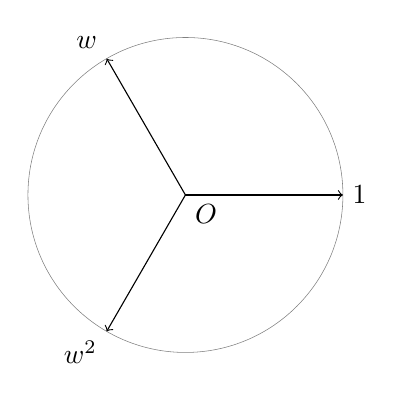
\begin{tikzpicture}[scale=2.0]
      \coordinate (A) at (1,0);
      \coordinate (B) at (120:1);
      \coordinate (C) at (240:1);
      \coordinate[label=below right:$O$] (O) at (0,0);
      \draw[help lines](0,0)circle(1);
      \tkzDrawPoint(O);
      \draw[->](O)--(A) node[pos=1,right]{$1$};
      \draw[->](O)--(B) node[pos=1,above left]{$w$};
      \draw[->](O)--(C) node[pos=1,below left]{$w^2$};
    \end{tikzpicture}
  \end{center}
  如上图,容易看出三个向量$1,w,w^2$的和是零向量。

  另一方面,由于$w^3=1$,从而对于任意整数$n$,$w^n, w^{n+1}, w^{n+2}$必是$1,w,w^2$这三者的某个排列,从而有
  \begin{align*}
    w^n + w^{n+1} + w^{n+2} = 0&\qedhere
  \end{align*}
\end{proof}

\begin{theorem}\label{th:equilateral-triangle-x+wy=0}
  复平面内两点$x,y$与原点组成正三角形,当且仅当
  \begin{align*}
    x + wy = 0
  \end{align*}
\end{theorem}
\begin{proof}[提示]
  $x+wy=0$的含义是将$y$旋转$120^\circ$后与$x$成反向量。
  \begin{center}
    \begin{tikzpicture}[scale=2.0]
      \coordinate[label=below:$O$] (O) at (0,0);
      \coordinate (A) at (20:1);
      \coordinate (B) at (80:1);
      \coordinate (C) at (200:1);
      \draw[help lines](O)circle(1) (A)--(B);
      \draw[->](O)--(A)node[right]{$x$};
      \draw[->](O)--(B)node[above]{$y$};
      \draw[->,dashed](O)--(C)node[left]{$wy$};
      \draw pic["$120^\circ$",<->,draw=orange,angle eccentricity=1.6,angle radius=.6cm]{angle=B--O--C};
      \tkzDrawPoint(O);
    \end{tikzpicture}
  \end{center}
  如上图,当且仅当$x$与$y$长度相等且夹角为$60^\circ$时,即当且仅当$wy=-x$时,$x,y$及原点$O$组成正三角形。
\end{proof}

\begin{theorem}\label{th:equilateral-triangle-z1+wz2+w2z3}
  复平面内三点$z_1,z_2,z_3$组成正三角形,当且仅当
  \begin{align*}
    z_1 + wz_2 + w^2z_3 = 0
  \end{align*}
\end{theorem}
\begin{proof}[提示]
  应用上一例中的记号$w$,有$1=-w-w^2$,从而
  \begin{align*}
    z_1 + wz_2 + w^2z_3 = 0 &\iff (-w-w^2)z_1 + wz_2 + w^2z_3 = 0 \\
                            & \iff w\left(z_2-z_1\right) + w^2\left(z_3-z_1\right) = 0\\
                            & \iff \left(z_2-z_1\right) + w\left(z_3-z_1\right) = 0
  \end{align*}
  于是将坐标原点移到$z_1$,在新坐标系下原$z_2,z_3$的坐标则变为了$z_2-z_1$及$z_3-z_1$,从而原命题变为
  \begin{quotation}
    复平面内两点$x,y$及原点组成正三角形,当且仅当
    \begin{align*}
      x + wy = 0
    \end{align*}
  \end{quotation}
  而这由定理~\ref{th:equilateral-triangle-x+wy=0}可得。
\end{proof}

\section{拿破仑三角形}
\label{sec:napoleon-triangle}

通常认为拿破仑定理是法国的著名军事家拿破仑·波拿巴(Napoleon Bonaparte)提出的。

\begin{theorem}[拿破仑定理,Napoleon' Theorem]\label{th:napoleon-theorem}
  任意三角形,以其三边分别向外做三个正三角形,则这三个正三角形的重心连线组成一个正三角形。此正三角形称为外拿破仑三角形。

  同样的,若以其三边分别向内做三个正三角形,则这三个正三角形的重心连线同样组成一个正三角形。此正三角形称为内拿破仑三角形。

  \begin{center}
    \begin{tikzpicture}[scale=1.0]
      \begin{scope}
        \coordinate[label=below left:$A$] (A) at (0,0);
        \coordinate[label=below right:$B$] (B) at (3,0);
        \coordinate[label=above:$C$] (C) at (2,2);
        \coordinate[label=below:$C'$] (C') at ($(B)!1!60:(A)$);
        \coordinate[label=above left:$B'$] (B') at ($(A)!1!60:(C)$);
        \coordinate[label=right:$A'$] (A') at ($(C)!1!60:(B)$);
        \coordinate[label=below:$D$] (D) at ($1/3*(A) + 1/3*(B) + 1/3*(C')$);
        \coordinate[label=right:$E$] (E) at ($1/3*(B) + 1/3*(C) + 1/3*(A')$);
        \coordinate[label=left:$F$] (F) at ($1/3*(C) + 1/3*(A) + 1/3*(B')$);
        \coordinate (D') at ($(A)!1!60:(D)$);
        \coordinate (E') at ($(B)!1!60:(E)$);
        \coordinate (F') at ($(C)!1!60:(F)$);
        \draw[help lines,dashed] (D)--(D') (E)--(E') (F)--(F');
        \draw[help lines,line width=2pt](A)--(C')--(B) (B)--(A')--(C) (C)--(B')--(A);
        \draw[line width=2pt](A)--(B)--(C)--cycle;
        \draw(D)--(E)--(F)--cycle (D')--(E')--(F')--cycle;
      \end{scope}
      \begin{scope}[shift={(5,0)}]
        \coordinate (A) at (0,0);
        \coordinate (B) at (3,0);
        \coordinate (C) at (2.2,.85);
        \coordinate (C') at ($(B)!1!-60:(A)$);
        \coordinate (B') at ($(A)!1!-60:(C)$);
        \coordinate (A') at ($(C)!1!-60:(B)$);
        \coordinate (D) at ($1/3*(A) + 1/3*(B) + 1/3*(C')$);
        \coordinate (E) at ($1/3*(B) + 1/3*(C) + 1/3*(A')$);
        \coordinate (F) at ($1/3*(C) + 1/3*(A) + 1/3*(B')$);
        \draw[help lines,line width=2pt](A)--(C')--(B) (B)--(A')--(C) (C)--(B')--(A);
        \draw[line width=2pt](A)--(B)--(C)--cycle;
        \draw(D)--(E)--(F)--cycle;
      \end{scope}
    \end{tikzpicture}
  \end{center}
\end{theorem}
\begin{proof}[提示]
  实际上,由于作一边向外与向内作的正三角形是关于此边对称的,从而由外拿破仑三角形的顶点分别以原三角形的三边作反射得到三个反射点,则此三点就是内拿破仑三角形的三个顶点。

  应用定理~\ref{th:equilateral-triangle-z1+wz2+w2z3},记图中各点在复平面内的坐标分别是$A$,$B$,$C$,$D$,$E$,$F$,$A'$,$B'$及$C'$,则由重心是三顶点的坐标平均值,有
  \begin{align*}
    D = \frac13\left(A+B+C'\right)\\
    E = \frac13\left(B+C+A'\right)\\
    F = \frac13\left(C+A+B'\right)
  \end{align*}
  从而(按$A,B,C$分组,带$'$或不带$'$,且每组要有系数$1,w,w^2$)
  \begin{align*}
    &D + wE + w^2F \\
    =\,& \frac13\left(A+B+C'\right)
    + \frac13\cdot w\left(B+C+A'\right)
       + \frac13\cdot w^2\left(C+A+B'\right)\\
    =\,&\frac13\left( A + wC + w^2B' \right) + \frac13\left( B + wA' + w^2C \right)
       + \frac13\left( C' + wB + w^2A \right)
  \end{align*}
  且对于三角正三角形$\triangle ABC'$,$\triangle BCA'$及$\triangle CAB'$,有
    \begin{align*}
    A + wC + w^2 B' = 0\\
    B + wA' + w^2 C = 0\\
    C' + wB + w^2 A = 0
  \end{align*}
  从而$D+wE+w^2F=0$,按定理~\ref{th:equilateral-triangle-z1+wz2+w2z3},$\triangle DEF$是正三角形。同样的,内拿破仑三角形也是正三角形。
\end{proof}

\begin{example}
  内外拿破仑三角形的重心与原三角形的重心重合。
\end{example}
\begin{proof}[提示]
  还是用复数。如定理~\ref{th:napoleon-theorem},有
  \begin{align*}
    D = \frac13\left(A+B+C'\right),\quad
    E = \frac13\left(B+C+A'\right),\quad
    F = \frac13\left(C+A+B'\right)
  \end{align*}
  同时,由于向量$BC'$是向量$BA$逆时针旋转$60^\circ$而得,从而有
  \begin{align*}
    C'-B=e^{\frac{\pi}6 i} (A-B) \quad\implies\quad C' = B + e^{\frac{\pi}6 i} (A-B)    
  \end{align*}
  同理可得
  \begin{align*}
    A' = C + e^{\frac{\pi}6 i} (B-C),\quad
    B' = A + e^{\frac{\pi}6 i} (C-A)
  \end{align*}
  从而有$A'+B'+C' = A+B+C$,代入,则有
  \begin{align*}
    D + E + F & = \frac13\left(A+B+C'\right) + \frac13\left(B+C+A'\right) + \frac13\left(C+A+B'\right) \\
              & = A + B + C
  \end{align*}
  从而外拿破仑三角形的重心$\frac13(D+E+F)$与原三角形的重心$\frac13(A+B+C)$重合。

  同理,内拿破仑三角形的重心与原三角形的重心重合。
\end{proof}


\begin{example}[美国,1956]
  在任意三角形的每边向外作顶角为$120^\circ$的等腰三角形,则这三个等腰三角形的三个顶点组成一个正三角形。
\end{example}
\begin{proof}[提示]
  此问题与拿破仑三角形类似,同样可以用复数解决。
  \begin{center}
    \begin{tikzpicture}[scale=1.0]
      \begin{scope}
        \coordinate[label=below left:$A$] (A) at (0,0);
        \coordinate[label=below right:$B$] (B) at (3,0);
        \coordinate[label=above:$C$] (C) at (2,2);
        \coordinate[label=below:$C'$] (C') at ($(B)!1/sqrt(3)!30:(A)$);
        \coordinate[label=above left:$B'$] (B') at ($(A)!1/sqrt(3)!30:(C)$);
        \coordinate[label=right:$A'$] (A') at ($(C)!1/sqrt(3)!30:(B)$);
        % \coordinate[label=below:$D$] (D) at ($1/3*(A) + 1/3*(B) + 1/3*(C')$);
        % \coordinate[label=right:$E$] (E) at ($1/3*(B) + 1/3*(C) + 1/3*(A')$);
        % \coordinate[label=left:$F$] (F) at ($1/3*(C) + 1/3*(A) + 1/3*(B')$);
        % \coordinate (D') at ($(A)!1!60:(D)$);
        % \coordinate (E') at ($(B)!1!60:(E)$);
        % \coordinate (F') at ($(C)!1!60:(F)$);
        % \draw[help lines,dashed] (D)--(D') (E)--(E') (F)--(F');
        \draw[help lines,line width=2pt](A)--(C')--(B) (B)--(A')--(C) (C)--(B')--(A);
        \draw[line width=2pt](A)--(B)--(C)--cycle;
        % \draw(D)--(E)--(F)--cycle (D')--(E')--(F')--cycle;
        \draw(A')--(B')--(C')--cycle;
      \end{scope}
    \end{tikzpicture}
  \end{center}
  如上图,记各点在复平面内的坐标分别为$A$,$B$,$C$,$A'$,$B'$及$C'$,则由三个顶角为$120^\circ$的等腰三角形$\triangle AC'B$,$\triangle BA'C$及$\triangle CB'A$,有
  \begin{align*}
    \begin{cases}
      A-C'=w(B-C')\\
      B-A'=w(C-A')\\
      C-B'=w(A-B')
    \end{cases}
    \implies
    \begin{cases}
      C' = \frac{A-wB}{1-w}\\
      A' = \frac{B-wC}{1-w}\\
      B' = \frac{C-wA}{1-w}
    \end{cases}
  \end{align*}
  上式中$A-C'=w(B-C')$是因为向量$\vec{C'A}$是向量$\vec{C'B}$逆时针旋转$120^\circ$而得,其余类似。从而
  \begin{align*}
    A' + wB' + w^2C' &= \frac{B-wC}{1-w} + w\cdot\frac{C-wA}{1-w} + w^2\cdot\frac{A-wB}{1-w}\\
                     &= \frac1{1-w}\left( (B-wC) + w(C-wA) + w^2(A-wB) \right)\\
                     &= \frac1{1-w}\left( B-wC + wC-w^2A + w^2A-w^3B \right)
  \end{align*}
  由$w^3=1$可知$A'+wB'+w^2C'=0$,从而$\triangle A'B'C'$是正三角形。
\end{proof}

\begin{example}[南京,1978]
  如图,$A_1,B_1,C_1$分别是三个正角形$\triangle ABC_2$,$\triangle BCA_2$及$\triangle CAB_2$的重心,则
  \begin{enumerate}
  \item $AA_2=BB_2=CC_2=\sqrt3 B_1C_1$;
  \item $\triangle A_1B_1C_1$是正三角形。
  \end{enumerate}
    \begin{center}
    \begin{tikzpicture}[scale=1.0]
      \begin{scope}[blend mode=multiply]
        \coordinate[label=below left:$A$] (A) at (0,0);
        \coordinate[label=below right:$B$] (B) at (3,0);
        \coordinate[label=above:$C$] (C) at (2,2);
        \coordinate[label=below:$C_2$] (C') at ($(B)!1!60:(A)$);
        \coordinate[label=above left:$B_2$] (B') at ($(A)!1!60:(C)$);
        \coordinate[label=right:$A_2$] (A') at ($(C)!1!60:(B)$);
        \coordinate[label=below left:$C_1$] (D) at ($1/3*(A) + 1/3*(B) + 1/3*(C')$);
        \coordinate[label=right:$A_1$] (E) at ($1/3*(B) + 1/3*(C) + 1/3*(A')$);
        \coordinate[label=left:$B_1$] (F) at ($1/3*(C) + 1/3*(A) + 1/3*(B')$);
        \coordinate (D') at ($(A)!1!60:(D)$);
        \coordinate (E') at ($(B)!1!60:(E)$);
        \coordinate (F') at ($(C)!1!60:(F)$);

        % \fill[color=red!20,opacity=.5](A)--(C)--(C')--cycle;
        % \fill[color=blue!20,opacity=.5](A)--(B)--(B')--cycle;
        
        % \draw[help lines,dashed] (D)--(D') (E)--(E') (F)--(F');
        \draw[help lines,line width=2pt](A)--(C')--(B) (B)--(A')--(C) (C)--(B')--(A);
        \draw[line width=2pt](A)--(B)--(C)--cycle;
        \draw(D)--(E)--(F)--cycle;% (D')--(E')--(F')--cycle;
        \draw(A)--(A') (B)--(B') (C)--(C');
      \end{scope}
      \begin{scope}[shift={(7,0)},blend mode=multiply]
        \coordinate[label=below left:$A$] (A) at (0,0);
        \coordinate[label=below right:$B$] (B) at (3,0);
        \coordinate[label=above:$C$] (C) at (2,2);
        \coordinate[label=below:$C_2$] (C') at ($(B)!1!60:(A)$);
        \coordinate[label=above left:$B_2$] (B') at ($(A)!1!60:(C)$);
        \coordinate[label=right:$A_2$] (A') at ($(C)!1!60:(B)$);
        \coordinate[label=below left:$C_1$] (D) at ($1/3*(A) + 1/3*(B) + 1/3*(C')$);
        \coordinate[label=right:$A_1$] (E) at ($1/3*(B) + 1/3*(C) + 1/3*(A')$);
        \coordinate[label=left:$B_1$] (F) at ($1/3*(C) + 1/3*(A) + 1/3*(B')$);
        \coordinate (D') at ($(A)!1!60:(D)$);
        \coordinate (E') at ($(B)!1!60:(E)$);
        \coordinate (F') at ($(C)!1!60:(F)$);

        \fill[color=red!20,opacity=.5](A)--(C)--(C')--cycle;
        \fill[color=blue!20,opacity=.5](A)--(B)--(B')--cycle;
        
        % \draw[help lines,dashed] (D)--(D') (E)--(E') (F)--(F');
        \draw[help lines,line width=2pt](A)--(C')--(B) (B)--(A')--(C) (C)--(B')--(A);
        \draw[line width=2pt](A)--(B)--(C)--cycle;
        \draw(D)--(E)--(F)--cycle;% (D')--(E')--(F')--cycle;
        \draw(A)--(A') (B)--(B') (C)--(C');
      \end{scope}
    \end{tikzpicture}
  \end{center}
\end{example}
\begin{proof}[提示]
  $A_1B_1C_1$是三角形$\triangle ABC$的外拿破仑三角形,从而是正三角形。

  将三角形$\triangle AC_2C$绕点$A$逆时针旋转$60^\circ$可得$\triangle ABB_2$,从而有$CC_2=BB_2$。同理可得$AA_2=BB_2=CC_2$。

  
  用余弦定理证明$AA_2=\sqrt3B_1C_1$。在$\triangle ACA_2$中,对角$\angle ACA_2$应用余弦定理,有
  \begin{align*}
    AA_2^2 &= AC^2 + A_2C^2 - 2AC\cdot A_2C\cdot\cos(C+\frac\pi6)\\
           &= AC^2 + BC^2 - 2AC\cdot BC\cdot\cos(C+\frac\pi6)
  \end{align*}
  其次,在$\triangle B_1AC_1$中,对角$\angle B_1AC_1$应用余弦定理,有
  \begin{align*}
    B_1C_1^2 & = B_1A^2 + C_1A^2 - 2B_1A\cdot C_1A\cdot \cos(A+30^\circ + 30^\circ) \\
             &= B_1A^2 + C_1A^2 - 2B_1A\cdot C_1A\cdot \cos(A+\frac\pi6)
  \end{align*}
  比较两式,一个有$\angle A$,一个有$\angle C$,不好比较。将$B_1C_1$换为$A_1B_1$,则有望将后式中的$\angle A$换为$\angle C$。对$\triangle A_1CB_1$中的$\angle C$应用余弦定理,有
  \begin{align*}
    A_1B_1^2 &= A_1C^2 + B_1C^2 - 2A_1C\cdot B_1C\cdot\cos(C + 30^\circ + 30^\circ)\\
             & = A_1C^2 + B_1C^2 - 2A_1C\cdot B_1C\cdot\cos(C + \frac\pi6)
  \end{align*}
  再由正三角形$\triangle BCA_2$及正三角形$\triangle ACB_2$,应用例~\ref{ex:radius-of-equilateral-triangle}的结论,有
  \begin{align*}
    A_1C = \frac{BC}{\sqrt3},\quad B_1C = \frac{AC}{\sqrt3}
  \end{align*}
  代入,则有
  \begin{align*}
    A_1B_1^2 = \frac13\left(BC^2 + AC^2 - 2 BC\cdot AC\cdot\cos(C + \frac\pi6)\right)
  \end{align*}
  比较$AA_2$的表达式,可知$AA_2^2 = 3A_1B_1^2$,从而有$AA_2=\sqrt3 A_1B_1$。由于外拿破仑三角形$\triangle A_1B_1C_1$是正三角形,从而有
  \begin{align*}
    AA_2=BB_2=CC_2=\sqrt3 A_1B_1 = \sqrt3 B_1C_1 = \sqrt3 C_1A_1
  \end{align*}
\end{proof}

\begin{theorem}[拿破仑点的推广]
  如图,任意三角形$\triangle ABC$,以三边为底边分别向外(或向内)作相似的三个等腰三角形形成六边形,则三条对角线$AX$,$BY$,$CZ$共点。
  \begin{center}
    \begin{tikzpicture}[scale=1.0]
      \begin{scope}
        \coordinate[label=left:$A$](A) at (0,0);
        \coordinate[label=right:$B$](B) at (3,0);
        \coordinate[label=above:$C$](C) at (2.5,2.5);
        \coordinate[label=above right:$X$](X) at ($(C)!.5/cos(30)!30:(B)$);
        \coordinate[label=above left:$Y$](Y) at ($(A)!.5/cos(30)!30:(C)$);
        \coordinate[label=below:$Z$](Z) at ($(B)!.5/cos(30)!30:(A)$);
        % \fill[color=red!20](A)--(B)--(Z)--cycle;
        % \fill[color=blue!20](B)--(C)--(X)--cycle;
        % \fill[color=yellow!20](C)--(A)--(Y)--cycle;
        \draw(A)--(B)--(Z)--cycle (B)--(C)--(X)--cycle (C)--(A)--(Y)--cycle;
        \draw(A)--(X) (B)--(Y) (C)--(Z);
      \end{scope}
      \begin{scope}[shift={(5,0)}]
        \coordinate[label=left:$A$](A) at (0,0);
        \coordinate[label=right:$B$](B) at (3,0);
        \coordinate[label=above:$C$](C) at (2.5,2.5);
        \coordinate[label=above right:$X$](X) at ($(C)!.5/cos(30)!30:(B)$);
        \coordinate[label=above left:$Y$](Y) at ($(A)!.5/cos(30)!30:(C)$);
        \coordinate[label=below:$Z$](Z) at ($(B)!.5/cos(30)!30:(A)$);
        \fill[color=red!20](A)--(B)--(Z)--cycle;
        \fill[color=blue!20](B)--(C)--(X)--cycle;
        \fill[color=yellow!20](C)--(A)--(Y)--cycle;
        \draw(A)--(B)--(Z)--cycle (B)--(C)--(X)--cycle (C)--(A)--(Y)--cycle;
        \draw(A)--(X) (B)--(Y);% (C)--(Z);
        \draw pic["$\theta$",<->,draw=orange,angle eccentricity=1.6,angle radius=.3cm]{angle=B--C--X};
        \draw pic["$\theta$",<->,draw=orange,angle eccentricity=1.6,angle radius=.3cm]{angle=X--B--C};
        \draw pic["$\theta$",<->,draw=orange,angle eccentricity=1.6,angle radius=.3cm]{angle=Z--A--B};
        \draw pic["$\theta$",<->,draw=orange,angle eccentricity=1.6,angle radius=.3cm]{angle=A--B--Z};
        \draw pic["$\theta$",<->,draw=orange,angle eccentricity=1.6,angle radius=.3cm]{angle=C--A--Y};
        \draw pic["$\theta$",<->,draw=orange,angle eccentricity=1.6,angle radius=.3cm]{angle=Y--C--A};
      \end{scope}
    \end{tikzpicture}
  \end{center}
  当$\theta=\pi/6$时,三线的交点即为first Napoleon point,也称为Fermat点;当$\theta=-\pi/6$时(即等腰三角形是向内的),三线的交点即为second Napoleon point。
\end{theorem}
% \begin{proof}[提示]
%   此定理的证明并不平凡,若有兴趣,可以参考Eddy, R. H.; Fritsch, R. (June 1994). "The Conics of Ludwig Kiepert: A Comprehensive Lesson in the Geometry of the Triangle". Mathematics Magazine. 67 (3): 188--205.
% \end{proof}

拿破仑点可以更进一步地推广如下,上面定理是下面定理的一种特殊情形。
\begin{theorem}[推广]
  给定任意三角形,如图在其三边向外作三个三角形$\triangle XBC$,$\triangle AYC$及$\triangle ABZ$,使得相邻的两个角相等,即
  \begin{align*}
    \angle YAC = \angle ZAB = \alpha,\quad
    \angle ZBA = \angle XBC = \beta,\quad
    \angle XCB = \angle YCA = \gamma
  \end{align*}
  则$AX$,$BY$及$CZ$三线共点,该点称为Jacobi点。
  \begin{center}
    \begin{tikzpicture}[scale=1.0]
      \coordinate[label=left:$B$] (B) at (0,0);
      \coordinate[label=right:$C$] (C) at (4,0);
      \coordinate[label=above:$A$] (A) at (3,2);
      % \coordinate[label=below:$X$] (X) at ($(C)!.8!30:(B)$);
      % \coordinate[label=below:$X$] (Y) at ($(C)!.8!-30:(A)$);
      % \tkzInterLL(A,X)(B,Y)\tkzGetPoint{N}
      % \tkzInterLL(C,N)(
      \coordinate(X1) at ($(B)!.5!-80:(C)$);\coordinate(X2) at ($(C)!.5!30:(B)$);\tkzInterLL(B,X1)(C,X2)\tkzGetPoint{X}
      \coordinate(Y1) at ($(A)!.5!60:(C)$);\coordinate(Y2) at ($(C)!.5!-30:(A)$);\tkzInterLL(A,Y1)(C,Y2)\tkzGetPoint{Y}
      \coordinate(Z1) at ($(A)!.5!-60:(B)$);\coordinate(Z2) at ($(B)!.5!80:(A)$);\tkzInterLL(A,Z1)(B,Z2)\tkzGetPoint{Z}
      \tkzInterLL(A,X)(B,C)\tkzGetPoint{X'}
      \tkzInterLL(B,Y)(C,A)\tkzGetPoint{Y'}
      \tkzInterLL(C,Z)(A,B)\tkzGetPoint{Z'}

      \draw pic["$\beta$",<->,draw=orange,angle eccentricity=1.8,angle radius=.3cm,fill=orange!20]{angle=X--B--C};
      \draw pic["$\beta$",<->,draw=orange,angle eccentricity=1.8,angle radius=.3cm,fill=orange!20]{angle=A--B--Z};

      \draw pic["$\gamma$",<->,draw=blue,angle eccentricity=1.6,angle radius=.5cm,fill=blue!20]{angle=B--C--X};
      \draw pic["$\gamma$",<->,draw=blue,angle eccentricity=1.6,angle radius=.5cm,fill=blue!20]{angle=Y--C--A};

      \draw pic["$\alpha$",<->,draw=red,angle eccentricity=1.6,angle radius=.3cm,fill=red!20]{angle=C--A--Y};
      \draw pic["$\alpha$",<->,draw=red,angle eccentricity=1.8,angle radius=.3cm,fill=red!20]{angle=Z--A--B};

      % \draw[help lines](X)--(Y)--(Z)--cycle;

      \draw(A)--(B)--(C)--cycle (B)--(X)--(C) (C)--(Y)--(A) (A)--(Z)--(B);
      \node[below] at (X) {$X$}; \node[above right] at (Y) {$Y$}; \node[above left] at (Z) {$Z$};
      \draw(A)--(X) (B)--(Y) (C)--(Z);
      \tkzInterLL(A,X)(B,Y)\tkzGetPoint{N}\tkzDrawPoint(N)
      % \node[label={[label distance=3pt]280:$N$}] at (N) {};
      \path (N) ++(.1,-.2) node[below]{$N$};
      \tkzDrawPoints(X',Y',Z')
      \path (X')++(.2,-.1)node[below]{$X'$};
      \path (Y')++(-.1,-.1)node[below]{$Y'$};
      \path (Z')++(-.1,0)node[left]{$Z'$};
    \end{tikzpicture}
  \end{center}
  $\triangle XYZ$称为$\triangle ABC$的一个Jacobi三角形。
\end{theorem}
\begin{proof}[提示]利用正弦定理及塞瓦定理。记三角形的三个顶角分别是$A,B,C$,对应的三条边长分别是$a,b,c$。

  考虑$\triangle AYY'$及$\triangle CYY'$,利用正弦定理,有
  \begin{align*}
    &\frac{\sin\angle AYY'}{AY'} = \frac{\sin\alpha}{YY'}, \quad
      \frac{\sin\angle CYY'}{Y'C} = \frac{\sin\gamma}{YY'}\\
    \implies& \frac{AY'}{Y'C} = \frac{\sin\alpha\cdot \sin\angle CYY'}{\sin\gamma\cdot\sin\angle AYY'}
  \end{align*}
  再对$\triangle AYB$和$\triangle CYB$应用正弦定理,有
  \begin{align*}
    &\frac{\sin\angle AYB}{c}=\frac{\sin(A+\alpha)}{BY},\quad
      \frac{\sin\angle CYB}{a}=\frac{\sin(C+\gamma)}{BY}\\
    \implies& \frac{\sin\angle AYB}{\sin\angle CYB}=\frac{a\sin(A+\alpha)}{c\sin(C+\gamma)}
  \end{align*}
  再由$\angle AYY' = \angle AYB$及$\angle CYY'=\angle CYB$,结合上面两式,有
  \begin{align*}
    \frac{AY'}{Y'C} = \frac{\sin\alpha\cdot c\cdot\sin(C+\gamma)}{\sin\gamma\cdot a\cdot\sin(A+\alpha)}
  \end{align*}
  同理可得出
  \begin{align*}
    \frac{CX'}{X'B}=\frac{\sin\gamma\cdot b\cdot\sin(B+\beta)}{\sin\beta\cdot c\cdot\sin(C+\gamma)},\quad
    \frac{BZ'}{Z'A}=\frac{\sin\beta\cdot a\cdot\sin(A+\alpha)}{\sin\alpha\cdot b\cdot\sin(B+\beta)}
  \end{align*}
  三式相乘,则有
  \begin{align*}
    \frac{AY'}{Y'C}\cdot\frac{CX'}{X'B}\cdot\frac{BZ'}{Z'A}=1
  \end{align*}
  由塞瓦定理,可知$AX'$,$BY'$,$CZ'$三线共点。
\end{proof}

\section{三角函数}
\label{sec:trigometric-functions}

\subsection{基本性质}
\label{sec:basic-properties-of-trigonometric-functions}

下面图中的圆是单位圆,当$0<\theta<90^\circ$时可在图中找到各基本三角函数的值。

\begin{center}
  \begin{tikzpicture}[scale=1.0]
    \coordinate[label=below left:$O$](O)at(0,0);
    \coordinate[label=above right:$C$](C)at(40:3);\coordinate(C1)at($(C)!.5!90:(O)$);
    \coordinate(A1)at(1,0);\coordinate(B1)at(0,1);
    \tkzInterLL(C,C1)(O,A1)\tkzGetPoint{A}\node[below right] at(A){$A$};
    \tkzInterLL(C,C1)(O,B1)\tkzGetPoint{B}\node[above]at(B){$B$};
    \coordinate[label=below:$D$](D)at($(O)!(C)!(1,0)$);
    \coordinate(E)at($(O)!(C)!(B)$);
    \draw[help lines](O)circle(3);
    \draw[dashed](C)--(E)node[pos=.55,above]{$\cos\theta$};
    \draw(A)--(D)
            --(O)node[midway,below]{$\cos\theta$}
            --(B)node[midway,left]{$\csc\theta$}
            --(C)node[midway,sloped,above]{$\cot\theta$}
            --(A)node[midway,sloped,above]{$\tan\theta$}
         (O)--(C)node[midway,above,sloped]{1}
            --(D)node[pos=.6,left]{$\sin\theta$};
    \tkzMarkRightAngle(A,O,B)\tkzMarkRightAngle(C,D,A)\tkzMarkRightAngle(O,C,B)\tkzMarkRightAngle(C,E,O)
    \tkzDrawPoints(O,A,B,C,D)
    \draw pic["$\theta$",<->,draw=orange,angle eccentricity=1.6,angle radius=.6cm]{angle=A--O--C};
    \draw[|<->|]($(O)-(0,1)$)--($(A)-(0,1)$)node[midway,fill=white]{$\sec\theta$};
  \end{tikzpicture}
\end{center}

由上图,根据勾股定理容易得到到一些性质:
\begin{gather*}
  \sin^2\theta + \cos^2\theta = 1,\quad \csc^2\theta=\cot^2\theta+1,\quad \sec^2\theta=\tan^2\theta+1\\
  \sec^2\theta+\csc^2\theta = (\cot\theta+\tan\theta)^2\\
  \tan^2\theta=\sin^2\theta+(\sec\theta-\cos\theta)^2\\
  \cot^2\theta=\cos^2\theta+(\csc\theta-\sin\theta)^2
\end{gather*}

\subsection{和差公式}
\label{sec:sum-and-difference-formula}

\begin{theorem}[和差公式,Sum and Difference Formulas]$\forall \alpha, \beta$,有
  \begin{align*}
    \sin(\alpha+\beta)=\sin\alpha\cos\beta + \cos\alpha\sin\beta\\
    \cos(\alpha+\beta)=\cos\alpha\cos\beta - \sin\alpha\sin\beta
  \end{align*}
\end{theorem}
\begin{proof}[提示]
  由下面的图,容易找到其中的关系。
  \begin{center}
    \begin{tikzpicture}[scale=1.0]
      \coordinate[label=below left:$O$](O)at(0,0);
      \coordinate[label=below right:$C$](C)at(5,0);
      \coordinate[label=right:$B$](B)at(5,1.8);
      \coordinate[label=above:$A$](A)at($(B)!.4!-90:(O)$);
      \coordinate[label=below:$D$](D)at($(O)!(A)!(C)$);
      \coordinate[label=above right:$E$](E)at($(C)!(A)!(B)$);
      \tkzMarkRightAngle(A,B,O)\tkzMarkRightAngle(B,C,O)\tkzMarkRightAngle(A,D,O)\tkzMarkRightAngle(A,E,B)
      \draw pic["$\alpha$",<->,draw=orange,angle eccentricity=1.6,angle radius=.6cm]{angle=C--O--B};
      \draw pic["$\beta$",<->,draw=orange,angle eccentricity=1.6,angle radius=.6cm]{angle=B--O--A};
      \draw pic["$\alpha$",<->,draw=orange,angle eccentricity=1.6,angle radius=.6cm]{angle=E--B--A};
      \draw(O)--(D)node[midway,below]{$\cos(\alpha+\beta)$}
              --(C)--(B)--(A)--(O)node[pos=.55,sloped,above right]{$1$}--(B);
      \draw[dashed](B)--(E)--(A)--(D);
      \draw[help lines,|<->|,sloped,above]($(E)+(1,0)$)--($(C)+(1,0)$)node[midway,color=black]{$\sin(\alpha+\beta)$};
      \tkzDrawPoints(O,A,B,C,D,E)
    \end{tikzpicture}
  \end{center}
  \begin{align*}
    \sin(\alpha+\beta) ={}& AD ={}& CB + BE ={}& \sin\beta\cos\alpha + \cos\beta\sin\alpha\\
    \cos(\alpha+\beta) ={}& OD ={}& OC - AE ={}& \cos\beta\cos\alpha - \sin\beta\sin\alpha &\qedhere
  \end{align*}
\end{proof}

\begin{example}
  用欧拉公式$e^{i\theta} = \cos\theta + i\sin\theta$证明和差公式。
\end{example}
\begin{proof}[提示]由欧拉公式,有
  \begin{align*}
    e^{i(\alpha + \beta)} = \cos(\alpha + \beta) + i\sin(\alpha + \beta)
  \end{align*}
  另一方面,由$e^{i(x+y)} = e^{ix}\cdot e^{iy}$,有
  \begin{align*}
    e^{i(\alpha + \beta)} ={}& e^{i\alpha}\cdot e^{i\beta}
    = \left( \cos\alpha + i\sin\alpha \right) \cdot \left( \cos\beta + i\sin\beta \right)\\
    ={}& (\cos\alpha\cos\beta - \sin\alpha\sin\beta) + i(\sin\alpha\cos\beta + \cos\alpha\sin\beta)
  \end{align*}
  对比两式,由虚部及实部分别相等,则有
  \begin{align*}
    \sin(\alpha+\beta) = \sin\alpha\cos\beta + \cos\alpha\sin\beta\\
    \cos(\alpha+\beta) = \cos\alpha\cos\beta - \sin\alpha\sin\beta    &\qedhere
  \end{align*}
\end{proof}

\begin{example}
  将和差公式中的$\beta$用$-\beta$替换,并注意到$\sin$与$\cos$的奇偶性,则有
  \begin{align*}
    \sin(\alpha-\beta) = \sin\alpha\cos(-\beta) + \cos\alpha\sin(-\beta) = \sin\alpha\cos\beta - \cos\alpha\sin\beta\\
    \cos(\alpha-\beta) = \cos\alpha\cos(-\beta) - \sin\alpha\sin(-\beta) = \cos\alpha\cos\beta + \sin\alpha\sin\beta
  \end{align*}
\end{example}

\begin{example}
  $\forall \alpha, \beta$,有
  \begin{align*}
    \tan\left(\frac{\alpha + \beta}{2}\right) = \frac{\sin\alpha + \sin\beta}{\cos\alpha + \cos\beta}
  \end{align*}
\end{example}
\begin{proof}[提示]
  由和差公式,容易得到
  \begin{align*}
    \sin(\alpha + \beta) + \sin(\alpha - \beta) ={}& 2 \sin\alpha\cos\beta \\
    \cos(\alpha + \beta) + \sin(\alpha - \beta) ={}& 2 \cos\alpha\cos\beta
  \end{align*}
  两式相除可得结论。
\end{proof}

\begin{theorem}
  $\forall \alpha,\beta$,有
  \begin{align*}
    \tan(\alpha+\beta) = \frac{\tan\alpha+\tan\beta}{1-\tan\alpha\tan\beta}
  \end{align*}
\end{theorem}
\begin{proof}[提示]
  利用和差公式,有
  \begin{align*}
    &\begin{cases}
      \sin(\alpha+\beta) = \sin\alpha\cos\beta + \cos\alpha\sin\beta\\
      \cos(\alpha+\beta) = \cos\alpha\cos\beta - \sin\alpha\sin\beta
    \end{cases}\\
    \implies& \tan(\alpha+\beta)=\frac{\sin(\alpha+\beta)}{\cos(\alpha+\beta)}
              =\frac{\sin\alpha\cos\beta + \cos\alpha\sin\beta}{\cos\alpha\cos\beta - \sin\alpha\sin\beta}
  \end{align*}
  分子分母同时除以$\cos\alpha\cos\beta$可得。此处没有考虑分母不能为零的情况。
\end{proof}

\begin{example}
  令$\tan(\alpha+\beta)=t$,则
  \begin{align*}
    t\cdot\tan\alpha\tan\beta + \tan\alpha + \tan\beta = t
  \end{align*}
  若$\alpha+\beta=30^\circ$,则$\tan(\alpha+\beta) = \frac{\sqrt3}{3}$,从而
  \begin{align*}
    \frac{\sqrt3}{3}\tan\alpha\tan\beta + \tan\alpha + \tan\beta = \frac{\sqrt3}{3}
  \end{align*}
  即
  \begin{align*}
    \tan\alpha\tan\beta + \sqrt3(\tan\alpha + \tan\beta) = 1
  \end{align*}
  如令$\alpha = 12^\circ$,$\beta = 30^\circ - \alpha = 18^\circ$,则有
  \begin{align*}
    \tan12^\circ\tan18^\circ + \sqrt3(\tan12^\circ + \tan18^\circ) = 1
  \end{align*}
\end{example}

\subsection{和差化积}
\label{sec:product-to-sum}

\begin{theorem}[和差化积,积化和差,Product-to-Sum Trigonometric Formulas]
  $\forall \alpha, \beta$,有
  \begin{align*}
    2\sin\alpha\sin\beta = \cos(\alpha-\beta) - \cos(\alpha+\beta)\\
    2\cos\alpha\cos\beta = \cos(\alpha-\beta) + \cos(\alpha+\beta)
  \end{align*}
\end{theorem}
\begin{proof}[提示]
  利用和差公式,有
  \begin{align*}
    \cos(\alpha-\beta) = \cos\alpha\cos\beta + \sin\alpha\sin\beta \\
    \cos(\alpha+\beta) = \cos\alpha\cos\beta - \sin\alpha\sin\beta
  \end{align*}
  两式相加及两式相减,则有
  \begin{align*}
    2\sin\alpha\sin\beta = \cos(\alpha-\beta) - \cos(\alpha+\beta) \\
    2\cos\alpha\cos\beta = \cos(\alpha-\beta) + \cos(\alpha+\beta)
  \end{align*}
  在不同场合,需要使用不同的形式,所以这些公式既叫和差化积,反过来也叫积化和差,是两个不同的方向。
\end{proof}

\begin{example}
  同样,利用$\sin$的和差公式,有
  \begin{align*}
    \sin(\alpha+\beta) = \sin\alpha\cos\beta + \cos\alpha\sin\beta \\
    \sin(\alpha-\beta) = \sin\alpha\cos\beta - \cos\alpha\sin\beta
  \end{align*}
  两式相加或相减,则有
  \begin{align*}
    2 \sin\alpha\cos\beta = \sin(\alpha + \beta) + \sin(\alpha - \beta)\\
    2 \cos\alpha\sin\beta = \sin(\alpha + \beta) - \sin(\alpha - \beta)&\qedhere
  \end{align*}
\end{example}

\begin{example}[和差化积公式互推]
  实际上,上述的和差化积公式都是可以互推的。比如,由$2\sin\alpha\sin\beta = \cos(\alpha-\beta) - \cos(\alpha+\beta)$,可得
  \begin{align*}
    \cos\alpha\cos\beta ={} & \sin(90^\circ - \alpha)\sin(90^\circ - \beta) \\
                        ={} & \cos\left( (90^\circ - \alpha) - (90^\circ - \beta) \right) - 
                              \cos\left( (90^\circ - \alpha) + (90^\circ - \beta) \right)\\
                        ={} & \cos(\beta - \alpha) - \cos\left( 180^\circ - (\alpha + \beta) \right) \\
                        ={} & \cos(\alpha - \beta) + \cos(\alpha + \beta)
  \end{align*}
  其余各式类似。可见,和差化积公式的本质还是和差公式,只要知道和差公式,和差化积公式很容易就能推导出来。
\end{example}

\begin{example}
  令$x \equiv \alpha - \beta$,$y\equiv \alpha + \beta$,则有
  \begin{align*}
    \alpha = \frac{y+x}{2},\quad \beta = \frac{y-x}{2}
  \end{align*}
  代入和差化积公式,则可以得到和差化积的另外一种形式:
  \begin{align*}
    \cos x - \cos y ={}& 2 \sin\frac{y+x}{2} \sin\frac{y-x}{2}\\[5pt]
    \cos x + \cos y ={}& 2 \cos\frac{y+x}{2} \cos\frac{y-x}{2}
  \end{align*}
  类似的,也有
  \begin{align*}
    \sin x + \sin y ={}& 2 \sin\frac{x+y}{2}\cos\frac{x-y}{2}\\[5pt]
    \sin x - \sin y ={}& 2 \cos\frac{x+y}{2}\sin\frac{x-y}{2}
  \end{align*}
\end{example}

\begin{example}\label{ex:sin(alpha-beta)=0}
  若$\sin\gamma\ne0$,则
  \begin{align*}
    \sin(\gamma-\alpha)\sin\beta = \sin(\gamma-\beta)\sin\alpha \iff
    \sin(\alpha - \beta) = 0
  \end{align*}
  若额外有$\sin\alpha\ne 0$,$\sin\beta\ne 0$,则有
  \begin{align*}
    \frac{\sin(\gamma-\alpha)}{\sin\alpha} = \frac{\sin(\gamma-\beta)}{\sin\beta} \iff
    \sin(\alpha - \beta) = 0
  \end{align*}
\end{example}
\begin{proof}[提示]
  应用公式$\sin(a + b) = \sin a \cos b + \sin b \cos a$,将$a= \gamma$、$b=-\alpha$及$a=\gamma$、$b=-\beta$代入,有
  \begin{align*}
    &&\sin(\gamma-\alpha)\sin\beta ={}& \sin(\gamma-\beta)\sin\alpha \\
    \iff &&
           \left(\sin\gamma\cos\alpha - \sin\alpha\cos\gamma\right) \sin\beta ={}& 
           \left(\sin\gamma\cos\beta -  \sin\beta \cos\gamma\right) \sin\alpha\\
    \iff&&
          \cos\alpha\sin\beta\sin\gamma - \cancel{\sin\alpha\sin\beta\cos\gamma}={}&
          \sin\alpha\cos\beta\sin\gamma - \cancel{\sin\alpha\sin\beta\cos\gamma}\\
    \iff&& \sin\gamma(\sin\alpha\cos\beta - \cos\alpha\sin\beta) ={}& 0\\
    \iff&& \sin\gamma\sin(\alpha-\beta) ={}& 0\\
    \iff&& \sin(\alpha - \beta) ={}& 0 & \qedhere
  \end{align*}
\end{proof}

\begin{example}
  $\forall x$,有
  \begin{align*}
    \frac{\cos x-\cos 3x}{\cos x+\cos 3x} = \tan x \tan 2x
  \end{align*}
\end{example}
\begin{proof}[提示]
  利用和差化积公式,有
  \begin{align*}
    \cos x - \cos 3x ={}& 2\sin\frac{x + 3x}{2} \sin\frac{3x-x}{2} = 2\sin2x\sin x\\
    \cos x + \cos 3x ={}& 2\cos\frac{x + 3x}{2} \cos\frac{3x-x}{2} = 2\cos2x\cos x
  \end{align*}
  两式相除可得。
\end{proof}

\subsection{倍角公式}
\label{sec:double-angle-formula}

\begin{theorem}[倍角公式]$\forall \alpha$,有
  \begin{align*}
    \sin 2\alpha ={}& 2\sin\alpha\cos\alpha\\
    \cos 2\alpha ={}& \cos^2\alpha - \sin^2\alpha = 2\cos^2\alpha - 1 = 1 - 2\sin^2\alpha\\[5pt]
    \tan 2\alpha ={}& \frac{2\tan\alpha}{1 - \tan^2\alpha}
  \end{align*}
\end{theorem}
\begin{proof}[提示]
  由和差公式可得。两式相除后分子分母同除以$\cos^2\alpha$,可得到$\tan2\alpha$关于$\tan\alpha$的表达式。
\end{proof}

\subsection{半角公式}
\label{sec:half-angle-formula}

\begin{theorem}[正弦余弦半角公式]$\forall \alpha$,有
  \begin{align*}
    \sin\frac\alpha2 ={} \pm\sqrt{\frac{1-\cos\alpha}2},\quad
    \cos\frac\alpha2 ={} \pm\sqrt{\frac{1+\cos\alpha}2}
  \end{align*}
\end{theorem}
\begin{proof}[提示]
  应用积化和差公式,有
  \begin{align*}
    2\sin\alpha\sin\alpha = \cos(\alpha - \alpha) - \cos(\alpha + \alpha) = 1 - \cos2\alpha
  \end{align*}
  化简可得$\sin$的半角公式。类似地可得$\cos$的半角公式。

  或者,由$\cos$的倍角公式,有
  \begin{align*}
    \cos\alpha = 1 - 2\sin^2\frac\alpha2, \quad \cos\alpha = 2\cos^2\frac\alpha2 - 1
  \end{align*}
  化简后可$\sin$与$\cos$的半角公式。
\end{proof}

\begin{theorem}[正切半角公式]$\forall \alpha$,有
  \begin{align*}
    \tan\frac{\theta}{2} ={}& \frac{\sin\theta}{1 + \cos\theta} = \frac{1 - \cos\theta}{\sin\theta} = \frac{\tan\theta}{\sec\theta + 1} = \frac{\sec\theta - 1}{\tan\theta} = \frac{1}{\csc\theta + \cot\theta}\\
                         ={}& \csc\theta - \cot\theta
  \end{align*}  
\end{theorem}
\begin{proof}[提示]
  考虑$\theta$是锐角的情况,作图,其中的圆是单位圆。
  \begin{center}
    \begin{tikzpicture}[scale=1.0]
      \coordinate[label=below:$O$](O)at(0,0);
      \coordinate[label=below:$A$](A)at(-4,0);
      \coordinate[label=below left:$B$](B)at(4,0);
      \coordinate[label=above right:$C$](C)at(40:4);
      \coordinate[label=below:$D$](D)at($(A)!(C)!(B)$);
      \coordinate(E1)at(0,4);
      \tkzInterLL(A,C)(O,E1)\tkzGetPoint{E}\node[above left]at(E){$E$};
      \coordinate(F1)at($(C)!1!90:(O)$);
      \tkzInterLL(C,F1)(O,E)\tkzGetPoint{F}\node[above]at(F){$F$};
      \tkzInterLL(C,F1)(O,B)\tkzGetPoint{G}\node[below]at(G){$G$};
      \coordinate(H1)at($(G)!.1!90:(C)$);\tkzInterLL(G,H1)(C,B)\tkzGetPoint{H}\node[below]at(H){$H$};

      \coordinate(P1)at($(G)!1!-90:(B)$);\tkzInterLL(G,P1)(A,C)\tkzGetPoint{P}\node[above right]at(P){$P$};

      \draw[help lines,dashed](B)arc(0:180:4);%(A)
      \draw pic["$\theta$",<->,draw=orange,angle eccentricity=1.6,angle radius=.6cm]{angle=D--O--C};
      \draw pic["$\theta$",<->,draw=orange,angle eccentricity=1.6,angle radius=.6cm]{angle=E--F--C};
      \draw pic["$\theta/2$",<->,draw=orange,angle eccentricity=1.8,angle radius=.8cm]{angle=D--A--C};
      \draw pic["\small$\frac\theta2$",<->,draw=orange,angle eccentricity=1.8,angle radius=.8cm]{angle=D--C--B};
      \draw pic["\small$\frac\theta2$",<->,draw=orange,angle eccentricity=1.8,angle radius=.8cm]{angle=B--C--G};
      \draw pic["$\frac{\pi-\theta}2$",draw=orange,angle eccentricity=1.6,angle radius=.5cm,fill=blue!20]{angle=C--E--F};
      \draw pic["$\frac{\pi-\theta}2$",draw=orange,angle eccentricity=1.6,angle radius=.5cm,fill=blue!20]{angle=F--C--E};
      \draw pic["",draw=orange,angle eccentricity=1.6,angle radius=.5cm,fill=blue!20]{angle=A--E--O};
      \draw pic["",draw=orange,angle eccentricity=1.6,angle radius=.25cm,fill=blue!20]{angle=H--B--G};
      \draw pic["",draw=orange,angle eccentricity=1.6,angle radius=.25cm,fill=blue!20]{angle=G--H--B};
      \draw pic["",draw=orange,angle eccentricity=1.6,angle radius=.25cm,fill=blue!20]{angle=C--B--D};
      \draw pic["",draw=orange,angle eccentricity=1.6,angle radius=.4cm,fill=blue!20]{angle=G--C--P};
      \draw pic["",draw=orange,angle eccentricity=1.6,angle radius=.4cm,fill=blue!20]{angle=C--P--G};

      \tkzMarkRightAngle(A,D,C)\tkzMarkRightAngle(B,C,A)\tkzMarkRightAngle(E,O,A)
      \tkzMarkRightAngle(O,C,F)\tkzMarkRightAngle(H,G,C)\tkzMarkRightAngle(P,G,A)
      \draw[dashed](C)--(P)--(G)node[midway,sloped]{\tiny |||};
      \draw[dashed](B)--(H)--(G)node[midway,sloped]{\tiny |};
      \draw[line width=1.5pt](E)--(O)node[pos=.57]{$\tan\frac\theta2$};
      \draw(A)--(O)node[midway,below]{$1$}
              --(D)node[midway,below]{$\cos\theta$}
              --(B)--(C)--(E)--(A)
           (O)--(C)node[midway,fill=white]{$1$}
              --(D)node[pos=.6,sloped,below]{$\sin\theta$};
      \draw(E)--(F)node[midway,sloped]{\tiny ||}
              --(C)node[midway,sloped]{\tiny ||}node[midway,sloped,above]{$\cot\theta$}
              --(G)node[midway,sloped,above]{$\tan\theta$} node[midway,sloped]{\tiny |||}
              --(B)node[midway,sloped]{\tiny |};

      \draw[dashed, help lines, |<->|]($(O) - (5,0)$)--($(F)-(5,0)$)node[midway,sloped,fill=white]{$\csc\theta$};
      \draw[dashed, help lines, |<->|]($(O) - (0,1.2)$)--($(B)-(0,1.2)$)node[midway,sloped,fill=white]{$1$};
      \draw[dashed, help lines, |<->|]($(O) - (0,2)$)--($(G)-(0,2)$)node[midway,sloped,fill=white]{$\sec\theta$};

      \tkzDrawPoints(O,A,B,C,D,E,F,G,H,P)
    \end{tikzpicture}
  \end{center}
  如图,有
  \begin{align*}
    EO = \tan\frac\theta2 = \frac{CD}{AD} = \frac{\sin\theta}{1 + \cos\theta}
  \end{align*}
  在上式中,分子分母同时除以$\cos\theta$,则有
  \begin{align*}
    \frac{\sin\theta}{1 + \cos\theta} = \frac{\tan\theta}{\sec\theta + 1}
  \end{align*}
  或者在$\triangle GCP$中,两底角相等均为$(\pi - \theta)/2$,从而$PG=CG=\tan\theta$,从而由$\triangle APG$可知
  \begin{align*}
    \tan\frac\theta2 = \frac{PG}{AG} = \frac{\tan\theta}{\sec\theta + 1}
  \end{align*}
  同时除以$\sin\theta$,则有
  \begin{align*}
    \frac{\sin\theta}{1 + \cos\theta} = \frac{1}{\csc\theta + \cot\theta}
  \end{align*}
  同时乘以$1-\cos\theta$并由$\sin^2\theta = (1+\cos\theta)(1-\cos\theta)$,则有
  \begin{align*}
    \frac{\sin\theta}{1 + \cos\theta} = \frac{1 - \cos\theta}{\sin\theta}
  \end{align*}
  或者由$\triangle CDB$,可知
  \begin{align*}
    \tan\frac\theta2 = \frac{DB}{DC} = \frac{1 - \cos\theta}{\sin\theta}
  \end{align*}

  容易知道$\triangle FEC$两底角相等均为$\frac\pi2 - \frac\theta2$,故$FE=FC=\cot\theta$,从而
  \begin{align*}
    \tan\frac\theta2 = EO = FO - FE = FO - FC = \csc\theta - \cot\theta
  \end{align*}
  同样,$\triangle GBH$中两底角相等均为$\frac\pi2 - \frac\theta2$,故$GH=GB=\sec\theta - 1$,从而
  \begin{align*}
    \tan\frac\theta2 = \frac{GH}{GC} = \frac{\sec\theta - 1}{\tan\theta}&\qedhere
  \end{align*}
\end{proof}

\begin{example}证明:
  \begin{align*}
    \left( \frac{1 - \tan\frac\theta2}{1 + \tan\frac\theta2} \right)^2 =
    \frac{1 - \sin\theta}{1+\sin\theta}, \quad
    \left( \tan\frac\theta2 \right)^2 = \frac{1-\cos\theta}{1+\cos\theta}
  \end{align*}
\end{example}
\begin{proof}[提示]
由
  \begin{align*}
    &\tan\frac\theta2 = \frac{1-\cos\theta}{\sin\theta}\\
    \implies&
    1 - \tan\frac\theta2 = \frac{\sin\theta - 1+\cos\theta}{\sin\theta},\quad
    1 + \tan\frac\theta2 = \frac{\sin\theta + 1-\cos\theta}{\sin\theta}
  \end{align*}
  两式相除,则有
  \begin{align*}
    \frac{1 - \tan\frac\theta2}{1 + \tan\frac\theta2} = 
    \frac{\sin\theta - 1+\cos\theta}{\sin\theta + 1-\cos\theta}
  \end{align*}
  两边平方,则有
  \begin{align*}
    &\left( \frac{1 - \tan\frac\theta2}{1 + \tan\frac\theta2} \right)^2 =
     \left( \frac{\sin\theta - 1+\cos\theta}{\sin\theta + 1-\cos\theta} \right)^2\\
    \implies&\left( \frac{1 - \tan\frac\theta2}{1 + \tan\frac\theta2} \right)^2 =
             \frac{2(1 - \sin\theta - \cos\theta + \sin\theta\cos\theta)}{2(1+\sin\theta-\cos\theta-\sin\theta\cos\theta)}\\
    \implies&\left( \frac{1 - \tan\frac\theta2}{1 + \tan\frac\theta2} \right)^2 =
             \frac{(1 - \sin\theta)(1 - \cos\theta)}{(1+\sin\theta)(1-\cos\theta)}\\
    \implies&\left( \frac{1 - \tan\frac\theta2}{1 + \tan\frac\theta2} \right)^2 =
             \frac{1 - \sin\theta}{1+\sin\theta}
  \end{align*}

  而由
  \begin{align*}
    \tan\frac\theta2 = \frac{\sin\theta}{1+\cos\theta} = \frac{1-\cos\theta}{\sin\theta}
  \end{align*}
  两式相乘,可得
  \begin{align*}
    \left(\tan\frac\theta2\right)^2 = \frac{1-\cos\theta}{1+\cos\theta}&\qedhere
  \end{align*}
\end{proof}

\begin{theorem}[万能公式]$\forall \alpha$,有
  \begin{align*}
    \sin\alpha = \frac{2\tan\frac\alpha2}{1+\tan^2\frac\alpha2}, \quad
    \cos\alpha = \frac{1-\tan^2\frac\alpha2}{1+\tan^2\frac\alpha2},\quad
    \tan\alpha = \frac{2\tan\frac\alpha2}{1-\tan^2\frac\alpha2}
  \end{align*}  
\end{theorem}
\begin{proof}[提示]
  利用倍角公式(和差公式的特殊情形),有
  \begin{align*}
    \sin\alpha ={}& 2\sin\frac\alpha2\cos\frac\alpha2
                    = \frac{2\sin\frac\alpha2\cos\frac\alpha2}{\cos^2\frac\alpha2 + \sin^2\frac\alpha2}
                    = \frac{2\tan\frac\alpha2}{1 + \tan^2\frac\alpha2}\\
    \cos\alpha={}& \cos^2\frac\alpha2 - \sin^2\frac\alpha2
                   =\frac{\cos^2\frac\alpha2 - \sin^2\frac\alpha2}{\cos^2\frac\alpha2 + \sin^2\frac\alpha2}
                   =\frac{1-\tan^2\frac\alpha2}{1+\tan^2\frac\alpha2}    
  \end{align*}
  两式相除,可得$\tan\alpha$关于$\tan\frac\alpha2$的表达式。
\end{proof}

\section{解三角形}
\label{sec:solving-triangle}

\begin{example}如图,求$\angle\alpha$。
  \begin{center}
    \begin{tikzpicture}[scale=1.0]
      \begin{scope}
        \coordinate(B) at (0,0);
        \coordinate(C) at (4,0);
        \coordinate(D1) at ($(B)!1!20:(C)$); \coordinate(D2) at ($(C)!1!-110:(B)$);\tkzInterLL(B,D1)(C,D2)\tkzGetPoint{D}
        \coordinate(P1)at($(C)!1!-40:(B)$);\coordinate(P2)at($(D)!1!-80:(C)$);\tkzInterLL(C,P1)(D,P2)\tkzGetPoint{P}
        \coordinate(A1)at($(B)!1!30:(P)$);\tkzInterLL(B,A1)(D,P)\tkzGetPoint{A}
        \coordinate(E1)at($(D)!1!-50:(P)$);\tkzInterLL(B,P)(D,E1)\tkzGetPoint{E}
        \tkzInterLL(C,P)(B,D)\tkzGetPoint{Q}
        \draw(A)--(B)--(C)--(D)--(E)--cycle;
        \draw(A)--(D) (D)--(B)--(E) (C)--(P);
        \tkzDrawPoints(A,B,C,D,E,P,Q)
        \node[left]at(A){$A$};
        \node[below left]at(B){$B$};
        \node[below right]at(C){$C$};
        \node[right]at(D){$D$};
        \node[above]at(E){$E$};
        \path (P)++(-.1,-.2)node[left]{$P$};
        \node[above]at(Q){$Q$};
        \draw pic["$30^\circ$",<->,draw=orange,angle eccentricity=1.6,angle radius=.6cm]{angle=P--B--A};
        \draw pic["$\alpha$",<->,draw=orange,angle eccentricity=1.6,angle radius=.6cm]{angle=D--B--P};
        \draw pic["$20^\circ$",<->,draw=orange,angle eccentricity=1.6,angle radius=.8cm]{angle=C--B--D};
        \draw pic["$40^\circ$",<->,draw=orange,angle eccentricity=1.6,angle radius=.6cm]{angle=P--C--B};
        \draw pic["$70^\circ$",<->,draw=orange,angle eccentricity=1.7,angle radius=.3cm]{angle=D--C--P};
        \draw pic["$50^\circ$",<->,draw=orange,angle eccentricity=1.8,angle radius=.4cm]{angle=B--D--C};
        \draw pic["$30^\circ$",<->,draw=orange,angle eccentricity=1.6,angle radius=.6cm]{angle=P--D--B};
        \draw pic["$50^\circ$",<->,draw=orange,angle eccentricity=1.6,angle radius=.6cm]{angle=E--D--P};
        \draw pic["$30^\circ$",<->,draw=orange,angle eccentricity=1.6,angle radius=.6cm]{angle=C--P--D};
        \draw pic["$\theta$",<->,draw=orange,angle eccentricity=1.6,angle radius=.6cm]{angle=D--A--E};
      \end{scope}
      \begin{scope}[shift={(8,0)}]
        \coordinate(B) at (0,0);
        \coordinate(C) at (4,0);
        \coordinate(D1) at ($(B)!1!20:(C)$); \coordinate(D2) at ($(C)!1!-110:(B)$);\tkzInterLL(B,D1)(C,D2)\tkzGetPoint{D}
        \coordinate(P1)at($(C)!1!-40:(B)$);\coordinate(P2)at($(D)!1!-80:(C)$);\tkzInterLL(C,P1)(D,P2)\tkzGetPoint{P}
        \coordinate(A1)at($(B)!1!30:(P)$);\tkzInterLL(B,A1)(D,P)\tkzGetPoint{A}
        \coordinate(E1)at($(D)!1!-50:(P)$);\tkzInterLL(B,P)(D,E1)\tkzGetPoint{E}
        \tkzInterLL(C,P)(B,D)\tkzGetPoint{Q}

        \coordinate[label=below:$F$](F) at ($(D)!1!60:(P)$);

        \draw pic["$30^\circ$",<->,draw=orange,angle eccentricity=1.6,angle radius=.6cm]{angle=P--B--A};
        \draw pic["$\alpha$",<->,draw=orange,angle eccentricity=1.6,angle radius=.6cm]{angle=D--B--P};
        \draw pic["$20^\circ$",<->,draw=orange,angle eccentricity=1.6,angle radius=.8cm]{angle=C--B--D};
        \draw pic["$40^\circ$",<->,draw=orange,angle eccentricity=1.6,angle radius=.6cm]{angle=P--C--B};
        \draw pic["$70^\circ$",<->,draw=orange,angle eccentricity=1.7,angle radius=.3cm]{angle=D--C--P};
        \draw pic["$50^\circ$",<->,draw=orange,angle eccentricity=1.8,angle radius=.4cm]{angle=B--D--C};
        \draw pic["$30^\circ$",<->,draw=orange,angle eccentricity=1.6,angle radius=.6cm]{angle=P--D--B};
        \draw pic["$50^\circ$",<->,draw=orange,angle eccentricity=1.6,angle radius=.6cm]{angle=E--D--P};
        \draw pic["$30^\circ$",<->,draw=orange,angle eccentricity=1.6,angle radius=.6cm]{angle=C--P--D};
        \draw pic["$\theta$",<->,draw=orange,angle eccentricity=1.6,angle radius=.6cm]{angle=D--A--E};

        \draw pic["",draw=blue,fill=blue!20,angle eccentricity=1.6,angle radius=.3cm]{angle=F--D--C};
        \draw pic["",draw=blue,fill=blue!20,angle eccentricity=1.6,angle radius=.5cm]{angle=C--F--D};
        \draw pic["",draw=blue,fill=blue!20,angle eccentricity=1.6,angle radius=.4cm]{angle=F--B--C};
        \draw pic["",draw=blue,fill=blue!20,angle eccentricity=1.6,angle radius=.4cm]{angle=C--B--D};

        \draw(A)--(B)--(C)--(D)--(E)--cycle;
        \draw(A)--(D) (D)--(B)--(E) (C)--(P);
        \tkzDrawPoints(A,B,C,D,E,P,Q)
        \node[left]at(A){$A$};
        \node[below left]at(B){$B$};
        \node[below right]at(C){$C$};
        \node[right]at(D){$D$};
        \node[above]at(E){$E$};
        \path (P)++(-.1,-.2)node[left]{$P$};
        \node[above]at(Q){$Q$};

        \draw[help lines, dashed](P)--(F)--(D) (C)--(F)--(B);
        \tkzDrawPoints(F)
      \end{scope}
    \end{tikzpicture}
  \end{center}
\end{example}
\begin{proof}[提示]
  首先,三角形$\triangle BCD$和$\triangle CDP$是固定的,从而四边形$BCDP$是固定的,即$\angle\alpha$是固定的,从而$\triangle BDA$及$\triangle BDE$也是固定的,即图形若有解的话,其解是唯一的。

  可以应用三角函数。容易知道$\angle BQP = 60^\circ$,$\angle BPQ = 120^\circ - \alpha$,从而应用正弦定理,有
  \begin{align*}
    \frac{\sin (120^\circ - \alpha)}{\sin\alpha} ={} &\frac{BQ}{PQ} = \frac{BQ}{CQ}\cdot\frac{CQ}{DQ}\cdot\frac{DQ}{PQ}\\
    ={}& \frac{\sin40^\circ}{\sin20^\circ}\cdot \frac{\sin50^\circ}{\sin70^\circ}\cdot \frac{\sin30^\circ}{\sin30^\circ}\\
    ={}& \frac{\sin40^\circ \sin50^\circ}{\sin20^\circ\sin70^\circ} = \frac{2\sin40^\circ \cos40^\circ}{2\sin20^\circ\cos20^\circ} = \frac{\sin80^\circ }{\sin40^\circ} \\
  \end{align*}
  比较两边,分子与分母的角度和都是$120^\circ$,可猜测$\alpha = 40^\circ$。事实上,由例~\ref{ex:sin(alpha-beta)=0},有
  \begin{align*}
    \sin(\alpha - 40^\circ) = 0
  \end{align*}
  从而$\alpha = 40^\circ + k\pi, k\in\mathcal{Z}$。又由$0 < \alpha < \pi$,可知$\alpha = 40^\circ$。

  或者用三角形全等来做。以$PD$为边,向$BC$方向做等边三角形$PDF$。如题图中的右图,可以找到几个全等的三角形:$\triangle PCF \cong \triangle PCD$(SAS,Side-Angle-Side,边角边),从而
  \begin{align*}
    &FC=DC\\
    \implies & \angle CFD = \angle CDF = 30^\circ + 50^\circ - 60^\circ = 20^\circ = CBD\\
    \implies & \text{从而$CFBD$四点共圆}\\
    \implies & \angle FBC = \angle FDC = 20^\circ\\
    \implies & \angle FBD = 20^\circ + 20^\circ = 40^\circ    
  \end{align*}
  此外,$\triangle BDP \cong \triangle BDF$(以$D$为顶点的SAS),从而
  \begin{align*}
    \alpha = \angle PBD = \angle FBD = 40^\circ &\qedhere
  \end{align*}
\end{proof}

\begin{example}
  上题中,$B$,$C$,$D$,$F$其实是正18边形的其中四个顶点。
  \begin{figure}[htbp]
    \centering
    \begin{tikzpicture}[scale=1.0]
      \coordinate[label=below left:$O$](O) at (0,0);
      \foreach \x in{0,1,2,3,4,5,6,7,8,9,10,11,12,13,14,15,16,17}{%
        \coordinate(V\x)at(360/18*\x:4.5);
        \tkzDrawPoint(V\x)
      }
      \foreach \x in{1,2,3,5,6,7,8,9,10,12,13,15,17}{%
        \node at(360/18*\x:5){$V_{\x}$};
      }
      \foreach \x in{0,11,14,16}{%
        \node at(360/18*\x:5.5){$(V_{\x})$};
      }
      \node[below right]at(V4){$V_4$};
      \draw[dashed, help lines](0,0)circle(4.5);
      \tkzDrawPoint(O)
      % \node[above right]at(V3){$V_3$};

      % \coordinate(B) at (0,0);
      % \coordinate(C) at (4,0);
      \coordinate(B) at (V11);\coordinate(C)at(V16);
      \coordinate(D1) at ($(B)!1!20:(C)$); \coordinate(D2) at ($(C)!1!-110:(B)$);\tkzInterLL(B,D1)(C,D2)\tkzGetPoint{D}
      \coordinate(P1)at($(C)!1!-40:(B)$);\coordinate(P2)at($(D)!1!-80:(C)$);\tkzInterLL(C,P1)(D,P2)\tkzGetPoint{P}
      \coordinate(A1)at($(B)!1!30:(P)$);\tkzInterLL(B,A1)(D,P)\tkzGetPoint{A}
      \coordinate(E1)at($(D)!1!-50:(P)$);\tkzInterLL(B,P)(D,E1)\tkzGetPoint{E}
      \tkzInterLL(C,P)(B,D)\tkzGetPoint{Q}

      \coordinate[label=below:$F$](F) at ($(D)!1!60:(P)$);

      \draw pic["$30^\circ$",<->,draw=orange,angle eccentricity=1.6,angle radius=.6cm]{angle=P--B--A};
      \draw pic["$\alpha$",<->,draw=orange,angle eccentricity=1.6,angle radius=.6cm]{angle=D--B--P};
      \draw pic["$20^\circ$",<->,draw=orange,angle eccentricity=1.6,angle radius=.8cm]{angle=C--B--D};
      \draw pic["$40^\circ$",<->,draw=orange,angle eccentricity=1.6,angle radius=.6cm]{angle=P--C--B};
      \draw pic["$70^\circ$",<->,draw=orange,angle eccentricity=1.7,angle radius=.3cm]{angle=D--C--P};
      \draw pic["$50^\circ$",<->,draw=orange,angle eccentricity=1.8,angle radius=.4cm]{angle=B--D--C};
      \draw pic["$30^\circ$",<->,draw=orange,angle eccentricity=1.6,angle radius=.6cm]{angle=P--D--B};
      \draw pic["$50^\circ$",<->,draw=orange,angle eccentricity=1.6,angle radius=.6cm]{angle=E--D--P};
      \draw pic["$30^\circ$",<->,draw=orange,angle eccentricity=1.6,angle radius=.6cm]{angle=C--P--D};
      \draw pic["$\theta$",<->,draw=orange,angle eccentricity=1.6,angle radius=.6cm]{angle=D--A--E};

      \draw pic["",draw=blue,fill=blue!20,angle eccentricity=1.6,angle radius=.3cm]{angle=F--D--C};
      \draw pic["",draw=blue,fill=blue!20,angle eccentricity=1.6,angle radius=.5cm]{angle=C--F--D};
      \draw pic["",draw=blue,fill=blue!20,angle eccentricity=1.6,angle radius=.4cm]{angle=F--B--C};
      \draw pic["",draw=blue,fill=blue!20,angle eccentricity=1.6,angle radius=.4cm]{angle=C--B--D};
      \draw pic["",draw=blue,fill=blue!20,angle eccentricity=1.6,angle radius=.4cm]{angle=O--D--B};

      \draw(A)--(B)--(C)--(D)--(E)--cycle;
      \draw(A)--(D) (D)--(B)--(E) (C)--(P);
      \tkzDrawPoints(A,B,C,D,E,P,Q)
      \node[below left]at(A){$A$};
      \node[below left]at(B){$B$};
      \node[below right]at(C){$C$};
      \node[right]at(D){$D$};
      \node[above]at(E){$E$};
      \path (P)++(-.1,-.2)node[left]{$P$};
      \node[above]at(Q){$Q$};

      \draw[help lines, dashed](P)--(F)--(D) (C)--(F)--(B);
      \tkzDrawPoints(F)

      \draw[dashed,help lines](V9)--(O)--(D) (V6)--(P)--(V7)--(A)--(V8);

      \tkzInterLL(C,P)(F,D)\tkzGetPoint{X}\tkzMarkRightAngle(Q,X,D)
    \end{tikzpicture}
    
    \caption{$BFCD$与正18边形}
    \label{fig:bfcd-and-18-polygon}
  \end{figure}

  如图~\ref{fig:bfcd-and-18-polygon},做$BFCD$的外接圆,不妨设此圆为单位圆。以$D$为第一个顶点$V_0$,逆时针找出外接圆上正18边形的其余17个顶点$V_i$,其中$(i=1,2,\cdots,17)$,则
  \begin{enumerate}
  \item $\angle DCB = 70^\circ + 40^\circ = 110^\circ\implies B$与$V_{11}$重合。
  \item $\angle FCD = 180^\circ - 20^\circ - 20^\circ = 140^\circ \implies F$与$V_{14}$重合。
  \item $\angle FCD = 140^\circ$且$FC=DC\implies C$与$V_{16}$重合。
  \item $\angle DCP = 70^\circ\implies CP$与圆相交于$V_7$。
  \item $DV_9$与$CV_7$都过圆心$\implies DV_0$与$CP$相交于外接圆的圆心$O$。
  \item 根据$\angle BDE=80^\circ$,可知$DE$与圆相交于$V_3$。
  \item 根据$\angle CBE=60^\circ$,可知$BE$与圆相交于$V_4$。
  \item 根据$\angle BDP=30^\circ$,可知$DP$与圆相交于$V_8$。
  \end{enumerate}
  其余性质不一一列举,有兴趣的可自行再去挖掘。
\end{example}

\begin{example}
  求上题中的$\angle\theta$。
\end{example}
\begin{proof}[提示]
  $\theta=50^\circ$,类似求$\alpha$,用三角函数求解。

  在$\triangle APE$中,由于$\angle APE = \angle BPD = 180^\circ - \alpha - 30^\circ = 110^\circ$,从而$\angle AEP = 70^\circ - \theta$。由正弦定理,有
  \begin{align*}
    &\frac{\sin\theta}{\sin\angle APE} = \frac{EP}{AP}\\[3pt]
    \implies&
        \frac{\sin\theta}{\sin(70^\circ -\theta)} =
        \frac{EP}{DP} \cdot \frac{DP}{BP} \cdot \frac{BP}{AP}\\
    \implies &
        \frac{\sin\theta}{\sin(70^\circ -\theta)} =
        \frac{\sin50^\circ}{\sin60^\circ} \cdot \frac{\sin40^\circ}{\sin30^\circ} \cdot \frac{\sin80^\circ}{\sin30^\circ}\\
    \implies &
        \sin60^\circ \sin30^\circ \sin30^\circ \sin\theta = \sin50^\circ\sin40^\circ\sin80^\circ\sin(70^\circ-\theta)\\
    \implies &
        \sqrt3\sin\theta = 8\cos40^\circ\sin40^\circ\sin80^\circ\sin(70^\circ-\theta)\\
    &\text{利用$\sin$的倍角公式}\\
    \implies & \sqrt3\sin\theta = 2\sin^280^\circ\sin(70^\circ-\theta)\\
    &\text{积化和差,} \sin\alpha\sin\alpha = \cos(\alpha-\alpha)-\cos(\alpha+\alpha) = 1-\cos2\alpha\\
    \implies & \sqrt3\sin\theta = 2(1-\cos160^\circ)\sin(70^\circ-\theta)\\
    \implies & \sqrt3\sin\theta = 2(1+\cos20^\circ)\sin(70^\circ-\theta)\\
    \implies & \sqrt3\sin\theta = 2\sin(70^\circ-\theta)+2\cos20^\circ\sin(70^\circ-\theta)\\
    \implies & \sqrt3\sin\theta = 2\sin(70^\circ-\theta)+\sin(20^\circ+70^\circ-\theta)-\sin(20^\circ-70^\circ+\theta)\\
    \implies & \sqrt3\sin\theta = 2\sin(70^\circ-\theta)+\cos\theta-\sin(\theta-50^\circ)\\
    \implies & \sqrt3\sin\theta -\cos\theta  = 2\sin(70^\circ-\theta)-\sin(\theta-50^\circ)\\
    &\text{和差公式}\\
    \implies & 2\sin(\theta-30^\circ) = 2\sin(70^\circ-\theta)-\sin(\theta-50^\circ)\\
    \implies & 2\left(\sin(\theta-30^\circ) -\sin(70^\circ-\theta)\right) + \sin(\theta-50^\circ) = 0\\
    &\text{和差化积}\\
    \implies & 4\cos20^\circ\sin(\theta-50^\circ) + \sin(\theta-50^\circ) = 0 \\
    \implies & \sin(\theta-50^\circ) = 0\\
    \implies & \theta = 50^\circ + k\pi,\quad k\in\mathcal{Z}
  \end{align*}
  又$0<\theta<\pi$,可知$\theta = 50^\circ$,即$AE=DE$。
\end{proof}